\documentclass[a4paper]{article}

\usepackage{fullpage} % Package to use full page
\usepackage{parskip} % Package to tweak paragraph skipping
\usepackage{tikz} % Package for drawing
\usepackage{amsmath}
\usepackage{hyperref}
\usepackage[utf8]{inputenc}
\usepackage{graphicx}
\usepackage{lmodern}
\usepackage[MeX]{polski}
\usepackage[T1]{fontenc}
\usepackage{float}

\title{Notatki z kursu Inżynieria Oprogramowania}
\author{Małgorzata Dymek}
\date{2018/19, semestr letni}

\begin{document}
    \maketitle


    \section{Wprowadzenie}
    \textbf{Inżynieria oprogramowania} - zastosowanie systematycznego, zdyscyplinowanego, ilościowego podejścia do rozwoju, eksploatacji i utrzymania
    oprogramowania, czyli zastosowanie \underline{inżynierskiego podejścia} do oprogramowania.
    Zagadnienia związanie z produkcją oprogramowania:
    \begin{itemize}
        \item analiza
        \item wymagania
        \item projektowanie
        \item wdrożenie
        \item ewolucja systemu
    \end{itemize}


    \subsection{Podstawowe pojęcia}
    \begin{itemize}
        \item Uczestnicy i \textbf{role}.
        \item \textbf{Systemy} i \textbf{modele}.
        \item \textbf{Produkt} - wewnętrzny lub docelowy.
        \begin{itemize}
            \item specyfikacja
            \item podręcznik użytkowania
            \item scenariusze przypadków użycia
            \item raport o statusie projektu
            \item podręcznik testera
        \end{itemize}
        \item \textbf{Aktywności}, zadania i \textbf{zasoby} - na przykład:
        \begin{itemize}
            \item zbieranie, analizowanie wymagań
            \item realizacja przypadku użycia
            \item zaprojektowanie schematu bazy danych, systemu, obiektów
            \item implementacja, testowanie
        \end{itemize}
        \textbf{Aktywności} służą zarządzaniu tworzeniem oprogramowania i używane są celem dostarczenia
        wysokiej jakoś produktu na czas i zgodnie z zaplanowanym budżetem. Koncentrują się na planowaniu
        projektu, monitorowaniu jego statusu, śledzeniu zmian i koordynowaniu wykorzystania zasobów.
        Obejmują m.in.:
        \begin{itemize}
            \item komunikację
            \item zarządzanie konfiguracją
            \item zarządzanie projektem
            \item cykl życiowy oprogramowania
        \end{itemize}
        \item \textbf{Notacje}, \textbf{metody} i \textbf{metodologie}.
        \item \textbf{Wymagania} - funkcjonalne i niefunkcjonalne.
    \end{itemize}




    \section {UML}

    \textbf{UML - Unified Modelling Language}
    \begin{itemize}
        \item rodzina \textbf{notacji} graficznych; unifikacja wielu obiektowych języków modelowania graficznego.
        \item służy do opisywania i projektowania stystemów informatycznych.
        \item nadzorowany przez organizacje OMG
        \item dwie podstawowe części:
        \begin{itemize}
            \item \textbf{Notacja} - składnia oraz elementy graficzne.
            \item \textbf{Metamodel} - semantyka oraz definicje pojęć języka i ich powiązań.
        \end{itemize}
    \end{itemize}
    \hfill \\
    \textbf{Sposoby użycia UML}:
    \begin{itemize}
        \item \textbf{Szkic}
        \begin{itemize}
            \item użyteczny podczas tworzenia i odtwarzania,
            \item charakter selektywny, nieformalny, dynamiczny.
        \end{itemize}
        \item \textbf{Projekt}
        \begin{itemize}
            \item użyteczny podczas tworzenia i odtwarzania,
            \item powinien być kompletny i zawierać wszystkie istotne decyzje,
            \item może dotyczyć tylko części systemu,
            \item wymaga bardziej skomplikowanych narzędzi niż szkic.
        \end{itemize}
        \item \textbf{Język programowania}
        \begin{itemize}
            \item diagramy tak szczegółowe, ze można generować kod automatycznie,
            \item wymaga bardzo skomplikowanych narzędzi.
        \end{itemize}
    \end{itemize}
    \hfill \\

    \textbf{Aktor} - użytkownik systemu; ogólnie wszystkie role, które wchodzą w interakcje z systemem, komponenty \underline{odpowiedzialne
    za incijalizację} use casów.

    \textbf{Scenariusz przypadku użycia} - wsypecyfikowana \underline{sekwencja zdarzeń} między użytkownikiem a systemem.
    \begin{itemize}
        \item Zdefiniowane w pierwszej kolejności.
        \item Wyróżnia się jeden \textbf{główny scenariusz sukcesu}.
        \item Może zawierać warunki wstępne, gwarancje lub wyzwalacze.
        \item W agile development używa się \underline{skróconej wersji scenariusza} odpowiadającej
        na pytania: kto, co, dlaczego.
    \end{itemize}

    \textbf{Przypadek użycia} - \underline{zbiór powiązanych ze sobą scenariuszy} opisujących użycie systemu przez aktorów.
    Opisujemy je tekstowo, poprzez user stories lub diagramy.
    \begin{itemize}
        \item reprezentuje \textbf{funkcjonalne wymaganie} systemu;
        \item pewna historia; opisuje akcje systemu z punktu widzenia użytkownika;
        \item specyfikuje jeden aspekt zachowania bez wchodzenia w strukturę systemu;
        \item jest zorientowany na osiągnięcie celu użytkownika;
    \end{itemize}
    Diagramy przypadków użycia są używane do modelowania kontekstu i wymagań systemu.

    \begin{figure}[h!]
        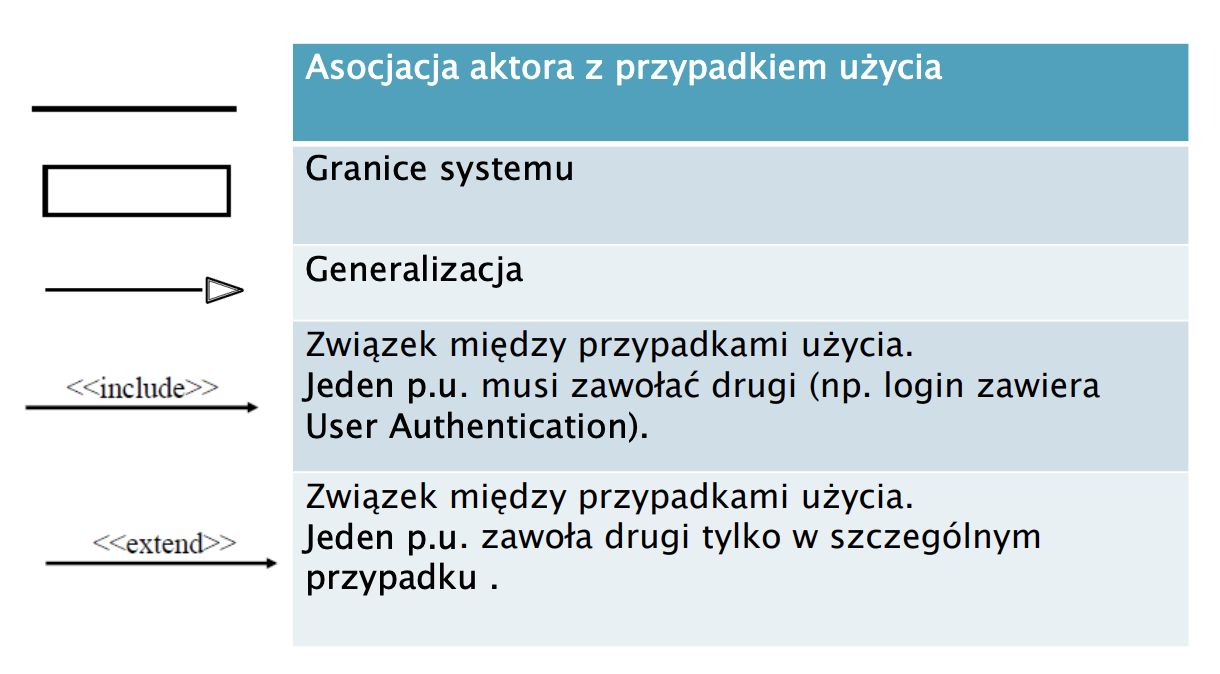
\includegraphics[width=\linewidth]{usecases.png}
    \end{figure}

    \textbf{Diagramy UML}

    \begin{tabular}{|c|c|}
        \hline
        Strukturalne & Behawioralne\\
        \hline
        diagram klas & diagram czynności\\
        diagram komponentów & diagram stanów\\
        diagram obiektów & diagram przypadków użycia\\
        diagram pakietów & diagram komunikacji\\
        diagram wdrożenia & diagram sekwencji\\
        diagram struktur złożonych & diagram przeglądu \\
        & diagram przebiegów czasowych\\
        \hline
    \end{tabular}


    \subsection{Diagram klas}
    \begin{itemize}
        \item jeden z najczęściej używanych, zwłaszcza do generowania kodu.
        \item struktura systemu w modelach obiektowych; ilustracja
        struktury klas i zależności między nimi,
        \item podział odpowiedzialności pomiędzy klasy i
        rodzaj wymienianych komunikatów,
    \end{itemize}

    \textbf{Klasy} służą do opanowania słownictwa tworzonego systemu. Używane do przedstawienia bytów programowych, sprzętowych,
    koncepcyjnych.
    \begin{itemize}
        \item simple names - $Customer$
        \item path names - $Business\_Rules::FraudAgent$
    \end{itemize}

    \begin{figure}[H]
        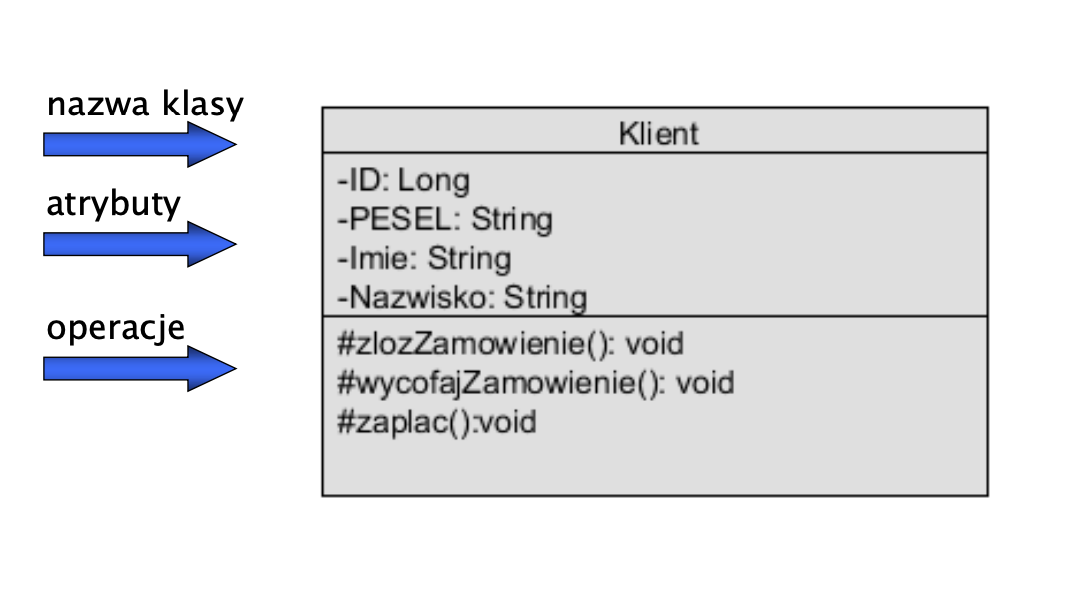
\includegraphics[width=\linewidth]{diagram_klasy.png}
    \end{figure}

    \begin{itemize}
        \item \textbf{Parametr} - przyjmowany przez metodę.
        \item \textbf{Atrybut} - nazwana właściwość klasy. Może mieć podaną klasę i wartość początkową.
        \begin{itemize}
            \item $+$  public
            \item \# protected
            \item $-$ private
        \end{itemize}
        \item \textbf{Operacja} (metoda) - implementacja pewnej usługi, której wykonania można zarządać
        od każdego obiektu klasy. Dokładne określenie przez podanie sygnatury (typy i domyślne wartości parametrów).
        \item \textbf{Odpowiedzialność} - wyrażenie zobowiązań klasy (lista).

        \item instance - każdy egzemplarz przechowuje oddzielną wartość
        \item classifier - jest tylko jedna wartość wspólna dla wszystkich egzemplarzy
        \item ilość wystąpień - liczba w prawym górnym rogu ($1 = singleton$)
    \end{itemize}
    \hfill \\
    \textbf{Związki pomiędzy klasami}

    \begin{figure}[H]
        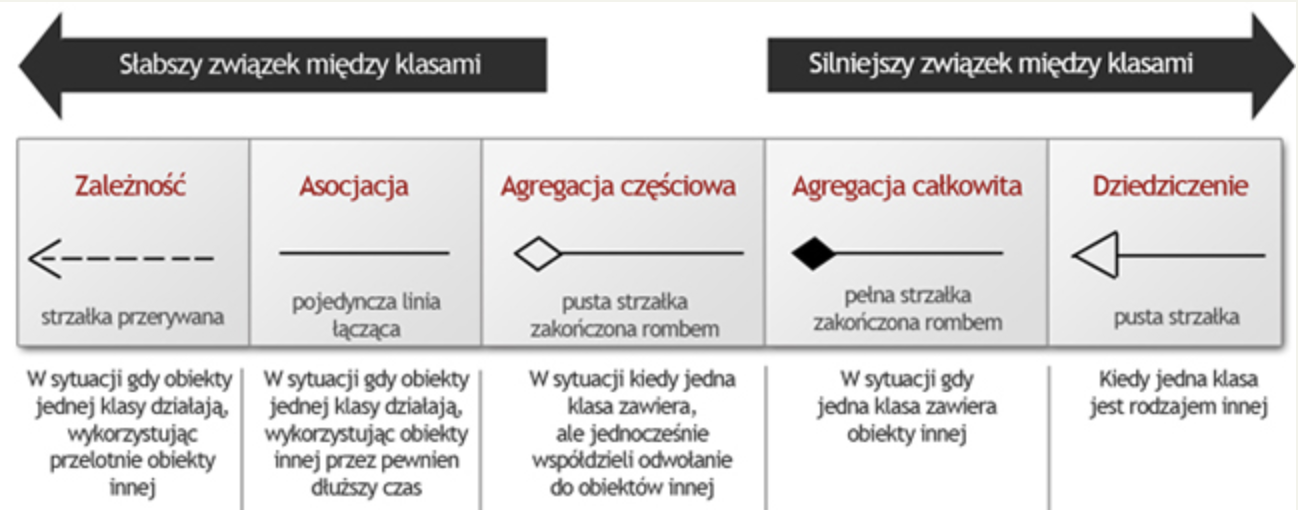
\includegraphics[width=\linewidth]{uml_zwiazki.png}
    \end{figure}

    Dodatkowo:
    \begin{itemize}
        \item \textbf{Implementacja} - linia przerywana
        zakończona pustą strzałką.
        \item \textbf{Rozszerzenia}
        \begin{itemize}
            \item \textbf{stereotypy} - służą do stworzenia nowego rodzaju obiektu ma podstawie innego obiektu
            będącego już w standardzie UML.
            \item \textbf{ograniczenia} - dotyczą zarówno klas jak i związków między nimi.
        \end{itemize}
        \item \textbf{Szablony} - klasy parametryzowane. Parametry szablony w prostokącie z przerywanych linii
        obok diagramu klasy.
    \end{itemize}


    \subsection{Procesy wytwarzania oprogramowania}
    Proces tworzenia oprogramowania - \textbf{zbiór czynności} i związanych z nimi wyników, \textbf{prowadzących do powstania
    systemu} informatycznego - tworzenie oprogramowania od zera, rozszerzanie i modyfikowanie istniejących systemów.

    \textbf{Cztery fundamentalne działania }wspólne dla wszystkich procesów:
    \begin{itemize}
        \item \textbf{Specyfikowanie} oprogramowania
        \begin{itemize}
            \item zebranie wymagań,
            \item definiowanie funkcjonalności i ograniczeń dotyczących
            tworzonego software’u.
        \end{itemize}
        \item \textbf{Tworzenie} oprogramowania
        \item \textbf{Walidacja} oprogramowania
        \item \textbf{Ewolucja} oprogramowania
    \end{itemize}

    \hfill \\
    \textbf{Cykl życia systemu} - cały okres istnienia systemu:
    \begin{itemize}
        \item studium zastosowalności
        \item analiza i specyfikacja,
        \item projektowanie i tworzenie,
        \item wdrażanie,
        \item pielęgnacja,
        \item aspekty usprawnienia.
    \end{itemize}

    \subsection{Modele procesu wytwarzania oprogramowania}
    \textbf{Model cyklu życia} systemu informatycznego ma na celu \underline{przedstawienie procesu} wytwarzania
    oprogramowania, który prowadzi do stworzenia działającego systemu.


    \subsubsection{Model kaskadowy}
    \begin{itemize}
        \item \textbf{wyizolowane etapy}, każdy musi być zakończony przed rozpoczęciem kolejnego
        \begin{itemize}
            \item \underline{Planowanie}: cele biznesowe, podstawowe wymagania, założenia, standardy, parametry,
            \item \underline{Analiza}: zdefiniowanie przeznaczenia systemu $\rightarrow$ kompletny, spójny i jednoznaczny model systemu,
            \item \underline{Projekt}: dekompozycja na podsystemy, wybór strategii budowania, projektowanie obiektów, wybór komponentów, opis interfejsów,
            \item \underline{Implementacja}: tworzenie kodu źródłowego, mapowanie modeli na kod,
            \item \underline{Testowanie}: znajdowanie różnic między rzeczywistym elementem a jego modelem,
            \item \underline{Pielęgnacja}.
        \end{itemize}
        \item Etapy podzielone na dwie części: \underline{twórczą} i \underline{weryfikacji}
        \item Ponowna praca, jeśli konieczna, jest wykonywana w kolejnych etapach - bardzo wysoki koszt błędów
        popełnionych we wstępnych etapach, adaptowanie zmian bardzo kosztowne.
        \item Koszty opracowania i akceptacji dokumentów są wysokie, powinien bvyć używany
        tylko jeśli wymagania są jasne i zrozumiałe.
        \item Marginalizacja roli klienta w procesie wytwarzania oprogramowania. Uzyskanie produktu zgodnego z wymaganiami
        silnie zależne od ich stabilności.
    \end{itemize}

    \subsubsection{Model V}
    \begin{figure}[H]
        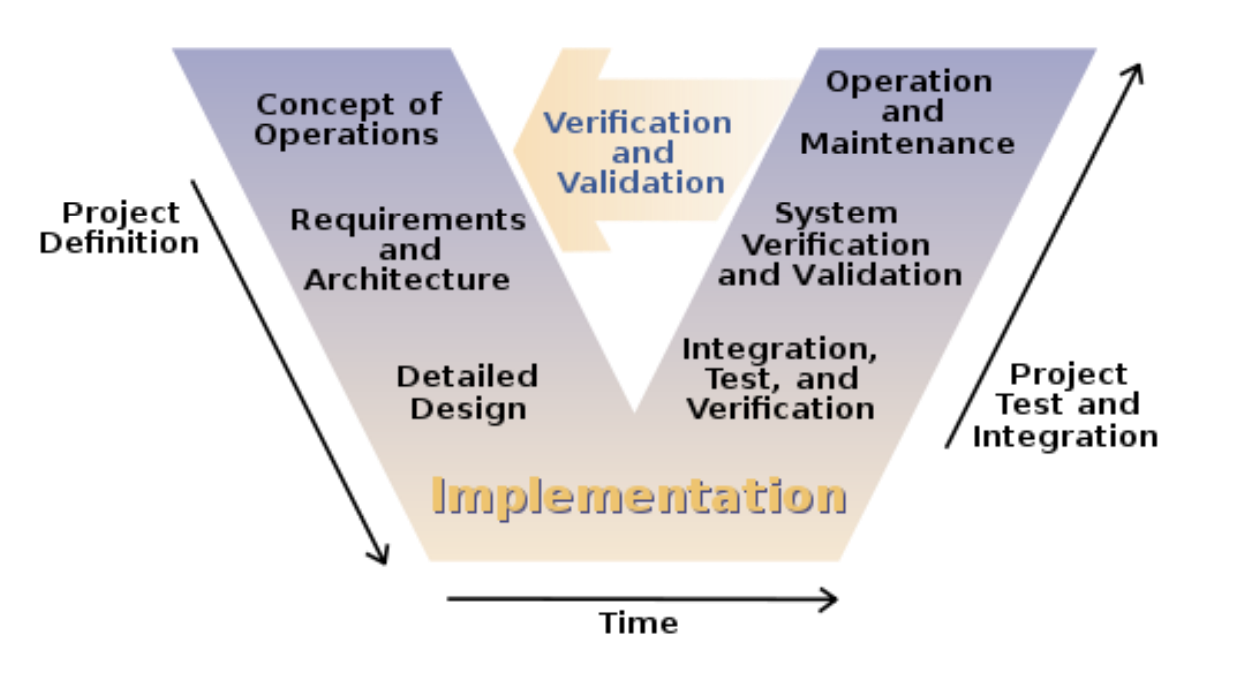
\includegraphics[width=\linewidth]{model_v.png}
    \end{figure}

    \subsubsection{Model Ewolucyjny}
    \begin{figure}[H]
        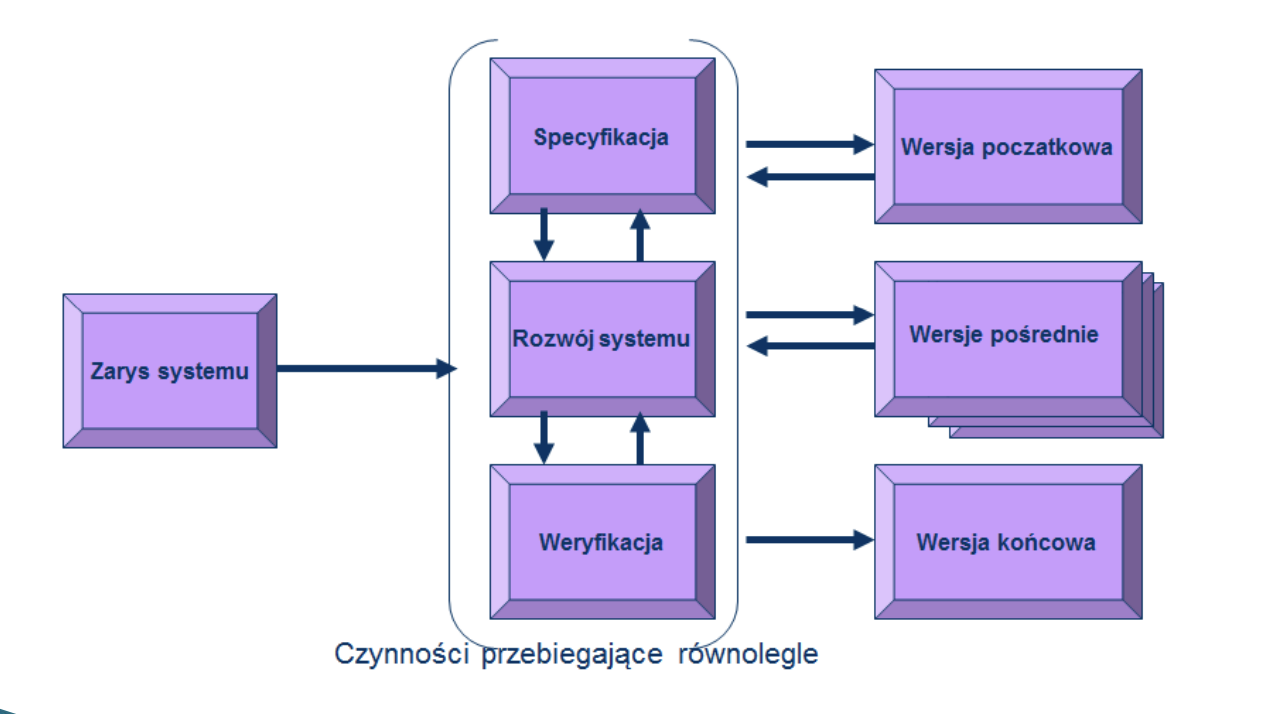
\includegraphics[width=\linewidth]{model_ewolucyjny.png}
    \end{figure}
    \begin{itemize}
        \item pozwala później określić wymagania do projektowanego systemu,
        \item prototyp pomaga kształcić przyszłego użytkownika,
        \item prototyp podnosi koszty w krótszej perspektywie, ale w
        dłuższej może je obniżać,
        \item zwykle prototyp jest wyrzucany.
    \end{itemize}

    \subsubsection{Model iteracyjny}
    \begin{figure}[H]
        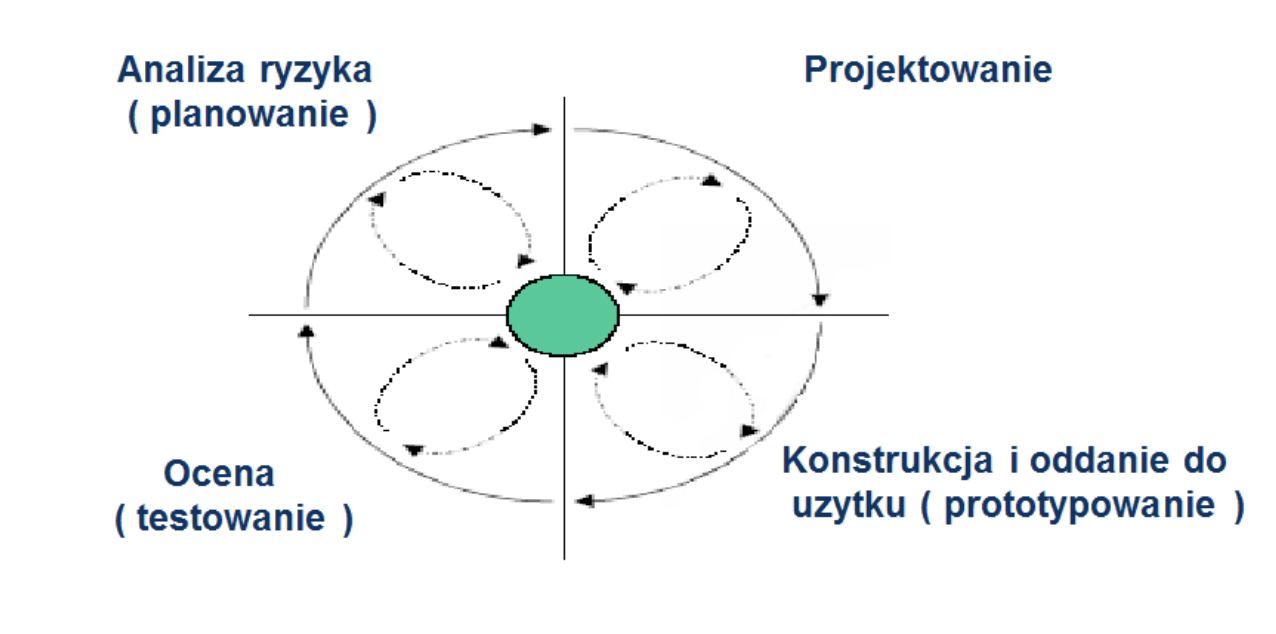
\includegraphics[width=\linewidth]{model_iteracyjny.png}
    \end{figure}
    \begin{itemize}
        \item pozwala na wczesne wykrywanie błędów,
        \item łączy iteracje z klasycznym modelem kaskadowym,
        \item łatwość wprowadzania zmian,
        \item wymogi klienta dotyczące harmonogramu mogą utrudnić korzystanie z tego
        modelu,
        \item problemy z oszacowaniem ryzyka.
    \end{itemize}

    \subsubsection{Model spiralny}
    \begin{figure}[H]
        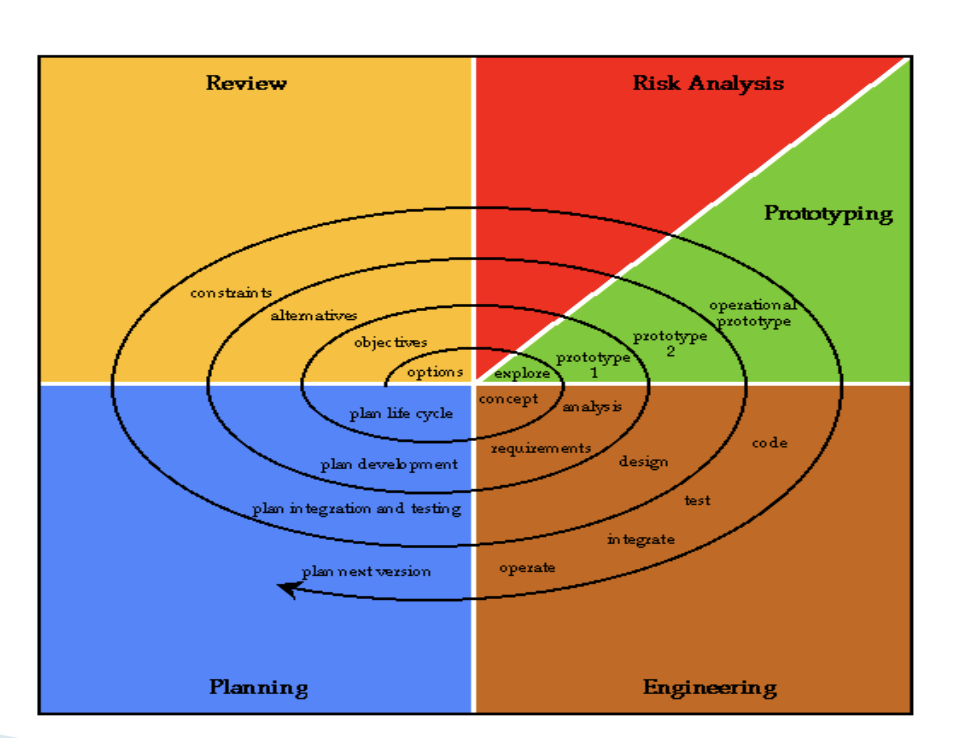
\includegraphics[width=\linewidth]{model_spiralny.png}
    \end{figure}
    \begin{itemize}
        \item ciągłe monitorowanie i pomiar zmian,
        \item zmiany poddawane są review użytkownika,
        \item próba minimalizacji ryzyka niepowodzenia.
    \end{itemize}

    \section{Standardy jakości}

    Odpowiedź na syndrom \textbf{LOOP} - \textbf{L}ate, \textbf{O}ver budget, \textbf{O}vertime, \textbf{P}oor quality.

    Minusy standaryzacji:
    \begin{itemize}
        \item Ważniejszy proces niż samo oprogramowanie,
        \item Spora cześć procesu jest fikcyjna, tworzenie dużej ilości dokumentacji,
        \item Dyscyplina zabija inicjatywę.
    \end{itemize}

    \subsection{CMM - Capability Maturity Model}
    Przeznaczony do \textbf{oceny procesu wytwórczego} służacego do produkcji oprogramowania.
    Ocena proces w skali pięciostopniowej - od chaotycznego (nic nie jest
    sterowane ani kontrolowane), aż do ścisłego, zdyscyplinowanego procesu uwzględniającego wszystkie potrzebne aspekty.

    Model CMM obejmuje \textbf{pięć aspektów}:
    \begin{itemize}
        \item Poziomy dojrzałości
        \item Kluczowe obszary procesowe
        \item Cele
        \item Atrybuty procesu
        \item Kluczowe praktywki
    \end{itemize}

    \subsubsection{Poziomy dojrzałości}
    \begin{itemize}
        \item \textbf{Poziom 1 - Wstępny}
        \begin{itemize}
            \item Działanie tymczasowe, doraźne.
            \item Organizacja bez stabilnej technologii wytwarzania i utrzymywania produktów.
            \item Zakres projektów zupełnie nieprzewidywalny.
        \end{itemize}
        \item \textbf{Poziom 2 - Powtarzalny}
        \begin{itemize}
            \item Dokumentowane standardy dokumentacji, szkoleń, utrzymywania.
            \item w miarę ustabilizowane środowisko pracy i procedury zarządzania.
        \end{itemize}
        \item \textbf{Poziom 3 - Zdefiniowany}
        \begin{itemize}
            \item Spójny zbiór definicji i standardów na poziomie
            organizacji realizującej projekt.
            \item Wyodrębnienie w zespole specjalistów od realizacji
            poszczególnych zadań, a organizacja dąży do wyposażenia ich
            w niezbędną wiedzę i umiejętności.
            \item Organizacja zaczyna na podstawie własnych doświadczeń
            modyfikować sposób prowadzenia projektów, tak aby
            maksymalnie odpowiadał jej specyfice.
        \end{itemize}
        \item \textbf{Poziom 4 - Zarządzany}
        \begin{itemize}
            \item W jakimś zdefiniowanym obszarze wyniki podejmowanych działań
            przenoszą określone rezultaty, które można zmierzyć za
            pomocą wcześniej zdefiniowanych metryk.
            \item Zadania, których wykonanie nie generuje dużej liczby
            błędów mogą być kontrolowane z mniejszą
            częstotliwością, zaś obszary zdefiniowane jako
            potencjalnie niebezpieczne np. w związku ze zmianą
            technologii, mogą podlegać ściślejszej kontroli.
        \end{itemize}
        \item \textbf{Poziom 5 - Optymalizujący}
        \begin{itemize}
            \item Proces jest już tak dobrze zorganizowany i zarządzany, że
            nie pozostaje nic innego, jak tylko dalsze podnoszenie
            stawianych przed procesem wymagań.
            \item Celem stawianym na tym poziomie jest optymalizacja i
            dalsze ulepszanie procesu, zwiększanie jego
            efektywności oraz wydajności.
        \end{itemize}
    \end{itemize}


    \subsection{ISO 9000}
    Jeden z najbardziej znanych standardów dotyczących jakości. Wymaga \textbf{udokumentowania wszystkich procedur} związanych z wytwarzaniem oprogramowania.

    \begin{figure}[H]
        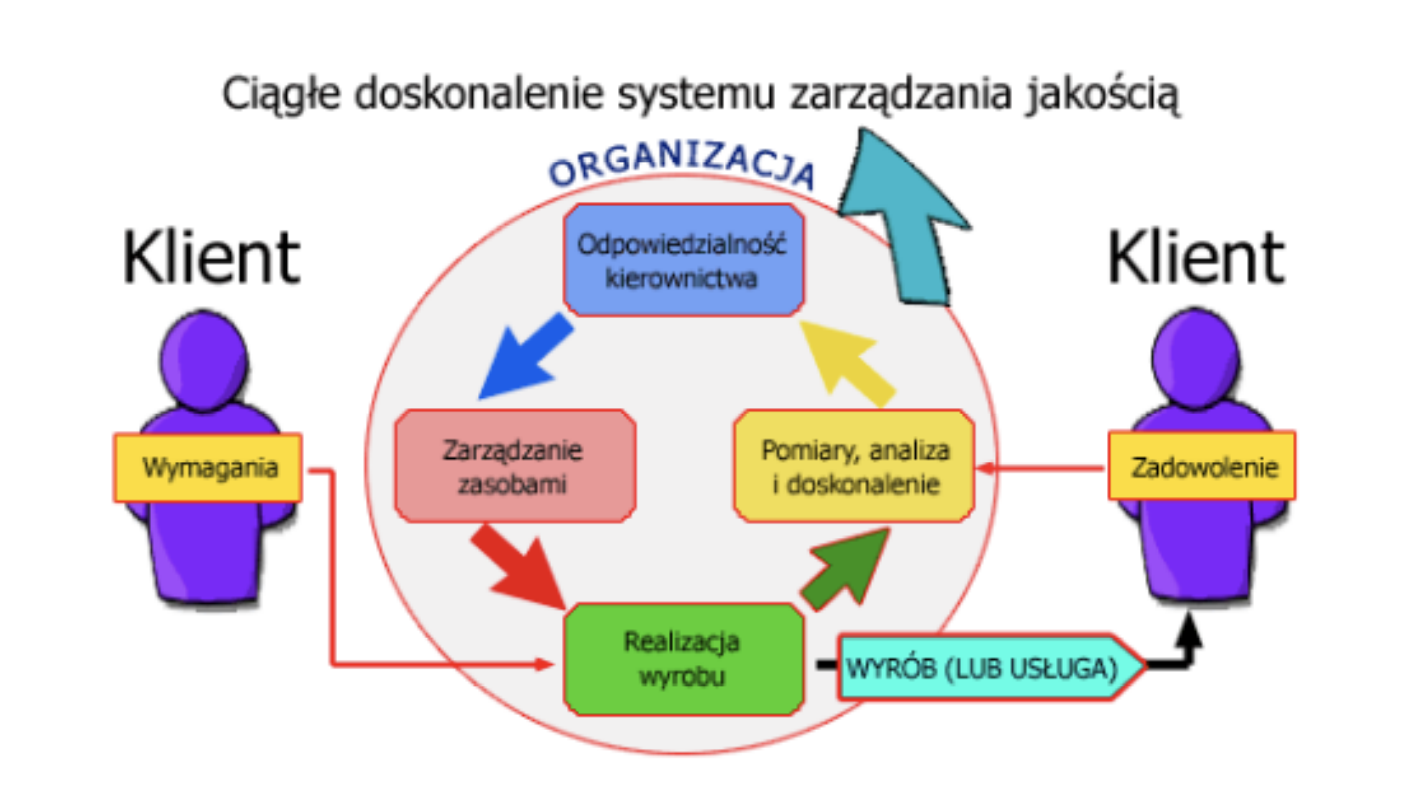
\includegraphics[width=\linewidth]{model_ISO.png}
    \end{figure}

    \begin{itemize}
        \item \textbf{Odpowiedzialność kierownictwa}\\
        Kierownictwo:
        \begin{itemize}
            \item odpowiada za właściwe funkcjonowanie organizacji,
            \item ustala misję i politykę organizacji, określa cele,
            \item opracowuje plan
            działań do realizacji celów i przyznaje odpowiednie zasoby.
        \end{itemize}
        \item \textbf{Zarządzanie zasobami}
        \begin{itemize}
            \item Zespół procesów związanych z zasobami - ludzkimi, infrastrukturą, środowiskiem pracy.
        \end{itemize}
        \item \textbf{Realizacja wyrobu}
        \begin{itemize}
            \item Zespół procesów bezpośrednio związany z
            realizacją wyrobu lub usługi.
            \item Wejściem są wymagania klienta, a wyjściem jest
            dostarczony wyrób lub usługa.
        \end{itemize}
        \item \textbf{Pomiary, analiza i doskonalenie}
        \begin{itemize}
            \item Procesy w organizacji i zadowolenie klienta
            wymagają systematycznego monitoringu, analizy i
            podejmowania działań doskonalących, aby wiedzieć
            jak postrzega nas klient (zadowolenie) oraz jak
            funkcjonują procesy w organizacji (zielona strzałka).
        \end{itemize}
        \item \textbf{Ciągłe doskonalenie} systemu zarządzania jakością
        \begin{itemize}
            \item Ciągłe zwiększanie skuteczności i efektywności w realizacji polityki,
            strategii i celów organizacji.
        \end{itemize}
    \end{itemize}

    \section{Zwinne procesy wytwarzania oprogramowania}
    Manifesto for Agile Software Development
    \begin{itemize}
        \item Individuals and interactions $\rightarrow$ Teamwork and responsibility
        \item Working software $\rightarrow$ Business value
        \item Customer collaboration $\rightarrow$ Partnership elaboration
        \item Respodning to change $\rightarrow$ Prepare for change
    \end{itemize}

    Lightweight (XP, Scrum) or fuller (DSDM, AUP) approaches.
    \textbf{Idea przepływu produktu przez system, podczas którego systematycznie zwiększana jest jego wartość.}

    \subsection{Programowanie ekstremalne - XP}
    \begin{figure}[H]
        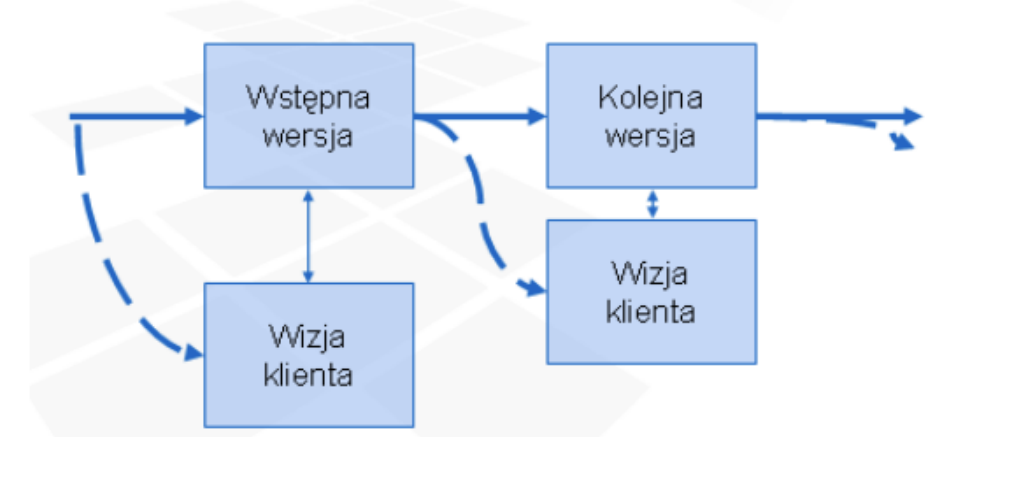
\includegraphics[width=\linewidth]{model_xp.png}
    \end{figure}

    Stawia na współpracę zespołu z klientem. Zakłada, że klient w dowolnym momencie może
    zmienić zdanie i zaproponować zmianę wymagań.
    Wady:
    \begin{itemize}
        \item brak fazy projektowania i dokumentacji,
        \item krótka perspektywa planowania,
        \item silne założenie, że klient pracuje cały czas z zespołem.
    \end{itemize}
    \hfill \\

    Projekt informatyczny - \textbf{szczelny systemem czterech zmiennych: daty dostarczenia, kosztu, liczby
    defektów oraz niekompletności funkcji}.

    Wartości:
    \begin{itemize}
        \item \textbf{Komunikacja} - przede wszystkim werbalna.
        \item \textbf{Prostota} - rozpoczynamy od najprostszego rozwiązania, spełniającego
        wymagania; refaktoryzacja pozwala na adaptacje oprogramowania do zmian.
        \item \textbf{Sprzężenie zwrotne} - obejmuje kilka aspektów (system, klient, zespół).
        \item \textbf{Odwaga} - potrzebna by: od razu produkować kod; refaktoryzować; wyrzucić zbędny kod.
        \item \textbf{Szacunek} - do pracy i czasu innych; między członkami zespołu.
    \end{itemize}

    \textbf{Struktura zespołu}
    \begin{itemize}
        \item \textbf{Role podstawowe}: programiści, klient,
        \item \textbf{Role pomocnicze}: tester, coach, tracker.
    \end{itemize}

    \textbf{User Stories}
    \begin{itemize}
        \item opisują \textbf{funkcje systemu} z punktu widzenia użytkownika,
        \item ważne by miały wartość dla klienta,
        \item powinny być testowane.
    \end{itemize}

    \textbf{Gra planistyczna}
    \begin{itemize}
        \item \textit{pisanie} user story (klient),
        \item \textit{oszacowanie} user story (informatycy),
        \item \textit{dzielenie} user story/wybór zakresu iteracji (klient).
    \end{itemize}

    \textbf{Zapewnianie jakości}
    \begin{itemize}
        \item prostota,
        \item unikanie optymalizacji,
        \item Test Driven Development - TTD,
        \item automatyczne testowanie,
        \item refaktoryzacja.
    \end{itemize}

    \textbf{Testy akceptacyjne}
    \begin{itemize}
        \item pochodzą od klienta (w ten sposób dokładnie określa,
        zachowanie systemu),
        \item najlepiej gdy mogą być wykonywane automatycznie (tester).
    \end{itemize}

    \textbf{Programowanie parami}
    \begin{itemize}
        \item zaleca się, by całość kodu pisana była w parach,
        \item częste zmiany w parach,
        \item wspólny standard kodowania,
        \item kod jest własnością całego zespołu,
        \item niezbędny system kontroli wersji.
    \end{itemize}

    \begin{figure}[H]
        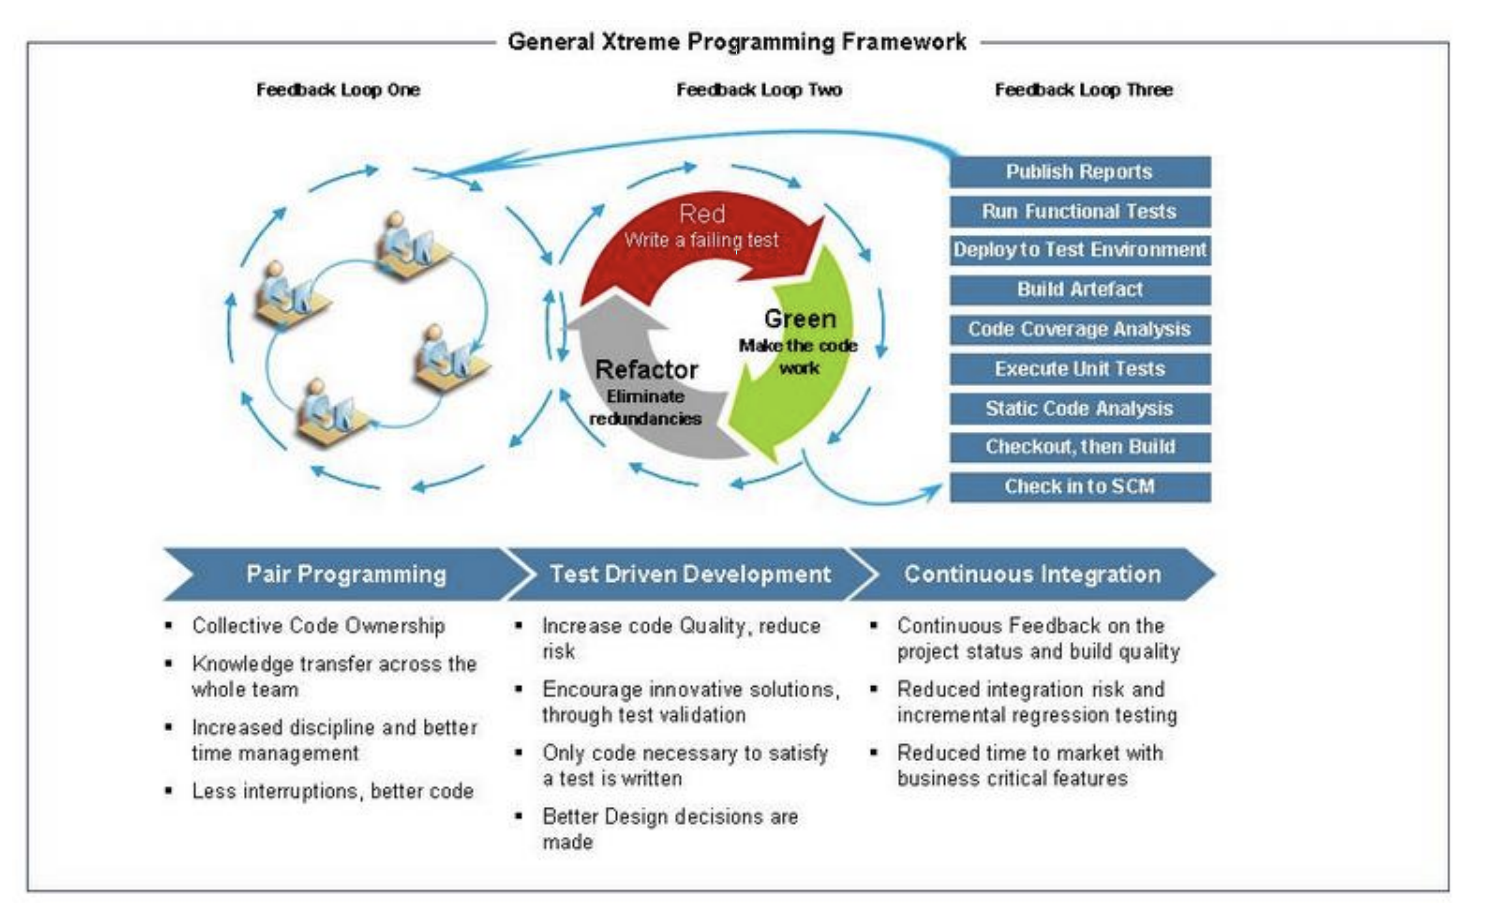
\includegraphics[width=\linewidth]{xp_framework.png}
    \end{figure}

    \subsection{SCRUM}
    Metoda przy użyciu której ludzie mogą z powodzeniem rozwiązywać \textbf{złożone problemy
    adaptacyjne}, by w sposób produktywny i kreatywny wytwarzać produkty o najwyższej możliwej wartości.
    \begin{itemize}
        \item lekki;
        \item łatwy do zrozumienia;
        \item bardzo trudny do opanowania.
    \end{itemize}

    \textbf{Trzy filary} teorii SCRUMa:
    \begin{itemize}
        \item \textbf{Adaptacja} - powinna być \underline{ciągła}. Korekta musi być
        wykonana jak najszybciej, by ograniczyć dalsze następstwa problemów.
        \item \textbf{Przejrzystość} - wszystkie \underline{istotne aspekty} procesu
        muszą być \underline{widoczne} dla osób odpowiedzialnych za osiągane rezultaty.
        \item \textbf{Inspekcja} – poddawane \underline{regularnej} inspekcji są zarówno scrumowe
        artefakty jak i postępy prac.
    \end{itemize}


    \textbf{Zdarzenia} - \textit{cztery formalne punkty} przeprowadzania inspekcji i dokonania korekty (adaptacji).

    \begin{tabular}{|c|c|c|}
        \hline
        ROLE & ARTEFAKTY & ZDARZENIA\\
        \hline
        Właściciel produktu & Przyrost Produktu & Sprint\\
        Zespół deweloperski & Rejestr Produktu & Planowanie Sprintu\\
        Scrum Master & Sprint Backlog & Codzienny Scrum\\
        & & Przegląd Sprint\\
        & & Retrospektywa Sprintu\\
        \hline
    \end{tabular}

    \subsubsection{Role w SCRUMie}
    \begin{itemize}
        \item \textbf{Właściciel Produktu} - odpowiedzialny za maksymalizację wartości produktu i pracy Zespołu
        Deweloperskiego. Jedyną osobą zarządzając Rejestrem Produktu co rozumiemy przez:
        \begin{itemize}
            \item jasne artykułowanie elementów Rejestru Produktu, określanie
            ich kolejności w sposób zapewniający osiąganie założonych celów i misji;
            \item zapewnianie dostępności i przejrzystości Rejestru Produktu dla wszystkich i to, że dobrze opisuje czym
            Zespół Scrumowy będzie się zajmował.
        \end{itemize}
        \item \textbf{Zespoł deweloperski}
        \begin{itemize}
            \item złożony z profesjonalistów (3-9 osób); samoorganizujący się, wielofunkcyjny.
            \item ma za zadanie dostarczenie (na zakończenie
            każdego Sprintu), gotowego do wydania Przyrostu produktu,
            \item nie przewiduje tytułów innych niż „Deweloper”,
            \item odpowiedzialność za wykonywaną pracę ponosi cały Zespół; brak podziału na podzespoły.
        \end{itemize}
        \item \textbf{Scrum Master}
        \begin{itemize}
            \item odpowiedzialny za to, by Scrum był rozumiany i stosowany,
            \item upewnia się, że Zespół Scrumowy stosuje się do założeń teorii Scruma, jego praktyk i reguł postępowania.
            \item wspiera zarówno Właściciela Produktu, jak i Zespól Deweloperski.
        \end{itemize}
    \end{itemize}

    \subsubsection{Zdarzenia w SCRUMie}
    \begin{itemize}
        \item ograniczone czasowo; używane do wprowadzenia regularności,
        \item każde (oprócz Sprintu) jest okazją do inspekcji i adaptacji.
        \\
        \item \textbf{Sprint} – serce Scruma
        \begin{itemize}
            \item stałe przez okres trwania prac ograniczenie czasowe trwające jeden miesiąc lub krócej;
            \item podczas Sprintu wytwarzany jest Przyrost ukończonej,
            używalnej i potencjalnie gotowej do wydania funkcjonalności,
            \item niedozwolone są zmiany, które wpłyną na cel Sprintu,
            \item niezmienny skład Zespołu Deweloperskiego i jego cel jakościowy.
        \end{itemize}
        \item \textbf{Przerwanie Sprintu}
        \begin{itemize}
            \item tylko Właściciel Produktu ma prawo to zrobić;
            \item w przypadku dezaktualizacji celu Sprintu,
            \item zużywa zasoby, bo powoduje przegrupowanie podczas kolejnego Planowania
            Sprintu.
        \end{itemize}
        \item \textbf{Planowanie Sprintu}
        \begin{itemize}
            \item ograniczone czasowo (8h/mies),
            \item Część pierwsza: \textit{Co będzie zrobione w tym Sprincie?}\\
            Wejście:
            \begin{itemize}
                \item Rejestr Produktu;
                \item ostatni przyrost;
                \item przewidywana pojemność ZD;
                \item ostatnie odczyty wydajności;
            \end{itemize}
            Wyjście:
            \begin{itemize}
                \item elementu Rejestru Produktu
                wybrane do zaimplementowania;
                \item cel Sprintu.
            \end{itemize}
            \item Część druga: \textit{Jak wybrana praca będzie wykonana?}\\
            \begin{itemize}
                \item zwykle rozpoczęcie od stworzenia projektu systemu i planu prac
               niezbędnych do przetworzenia elementów Rejestru Produktu w działający Przyrost produktu.
                \item zanim Planowanie Sprintu dobiegnie końca, ZD powinien móc wytłumaczyć Właścicielowi
            Produktu i Scrum Masterowi, w jaki sposób ma zamiar pracować, organizując się samodzielnie, by osiągnąć Cel
            Sprintu i wytworzyć oczekiwany Przyrost.
            \end{itemize}
        \end{itemize}
        \item \textbf{Codzienny Scrum} - spotkanie ograniczon do 15 minut, w którym każdy z
        członków zespołu wyjaśnia:
        \begin{itemize}
            \item Co zostało wykonane od ostatniego potkania?
            \item Co zostanie wykonane przed kolejnym spotkaniem?
            \item Jakie przeszkody stoją na drodze?
        \end{itemize}
        \item \textbf{Przegląd Sprintu} - max 4h, na zakończenie
        Sprintu w celu przeprowadzenia inspekcji Przyrostu i dostosowaniu, jeśli zajdzie taka
        potrzeba, Rejestru Produktu. Omówienie tego, co zostało ukończone w Sprincie.
        \begin{itemize}
            \item Właściciel Produktu stwierdza, które funkcjonalności zostały
            „Ukończone”, a które nie;
            \item Zespół Deweloperski omawia, co poszło dobrze w trakcie
            Sprintu; jakie były problemy i jak je rozwiązano;
            \item Zespół Deweloperski prezentuje „Ukończoną” pracę i
            odpowiada na pytania dotyczące Przyrostu,
            \item Właściciel Produktu omawia Rejestr Produktu w aktualnej
            jego postaci. Przewiduje termin zakończenia prac.
            \item Cala grupa omawia kolejne kroki.
        \end{itemize}
        \item \textbf{Retrospektywa Sprintu} - okazja do przeprowadzenia inspekcji
        swoich działań i opracowania planu usprawnień.
        \begin{itemize}
            \item Sprawdzenie, co działo się w ostatnim Sprincie, biorąc pod
            uwagę ludzi, zależności, procesy i narzędzia;
            \item Zidentyfikowanie i uporządkowanie istotnych elementów, które
            sprawdziły się w działaniu oraz tych, które kwalifikują się do
            poprawy;
            \item Stworzenie planu wprowadzania w życie usprawnień sposobu
            wykonywania pracy przez Zespół Scrumowy.
        \end{itemize}
    \end{itemize}

    \subsubsection{Artefakty}
    \begin{itemize}
        \item \textbf{Rejestr Produktu} - uporządkowana lista wszystkiego,
        co może być potrzebne w produkcie oraz jedyne źródło wymaganych zmian.
        Odpowiedzialny za RP jest Właściciel Produktu.
        Elementy posiadają atrybuty: opis, kolejność i oszacowanie (estymację).
        \item \textbf{Rejestr Sprintu} - podzbiór elementów RP wybranych do Sprintu rozszerzony o plan
        dostarczenia Przyrostu produktu.
        RS definiuje pracę, jaką ZD wykona by przekształcić elementy
        RP w „Ukończony” Przyrost.
        RS jest dobrze widocznym, tworzonym w czasie rzeczywistym obrazem pracy, jaką ZD planuje wykonać w trakcie Sprintu.
        RS należy tylko i wyłącznie do ZD.
        \\
        \item \textbf{Monitorowanie postępów Sprintu} – możliwe w każdym momencie Sprintu (Codzienny Scrum).
        \item \textbf{Przyrost} - suma wszystkich elementów RP zakończonych podczas wszystkich spirntów.
        Na koniec Sprintu nowy Przyrost musi być „Ukończony”.
        \item Aby zapewnić przejrzystość, wszyscy członkowie danego zespołu muszą mieć wspólne
        pojmowanie, co to znaczy, że praca jest skończona. Pomaga w tym \textbf{Definicja Ukończenia}
        dla Zespołu Scrumowego. W miarę dojrzewania Zespołu Scrumowego oczekuje się, że ich Definicja Ukończenia będzie
        zawierała coraz bardziej rygorystyczne kryteria zapewniania jeszcze wyższej jakości.
    \end{itemize}

    \subsection{AGILE PM (DSDM Atern)}

    \begin{figure}[H]
        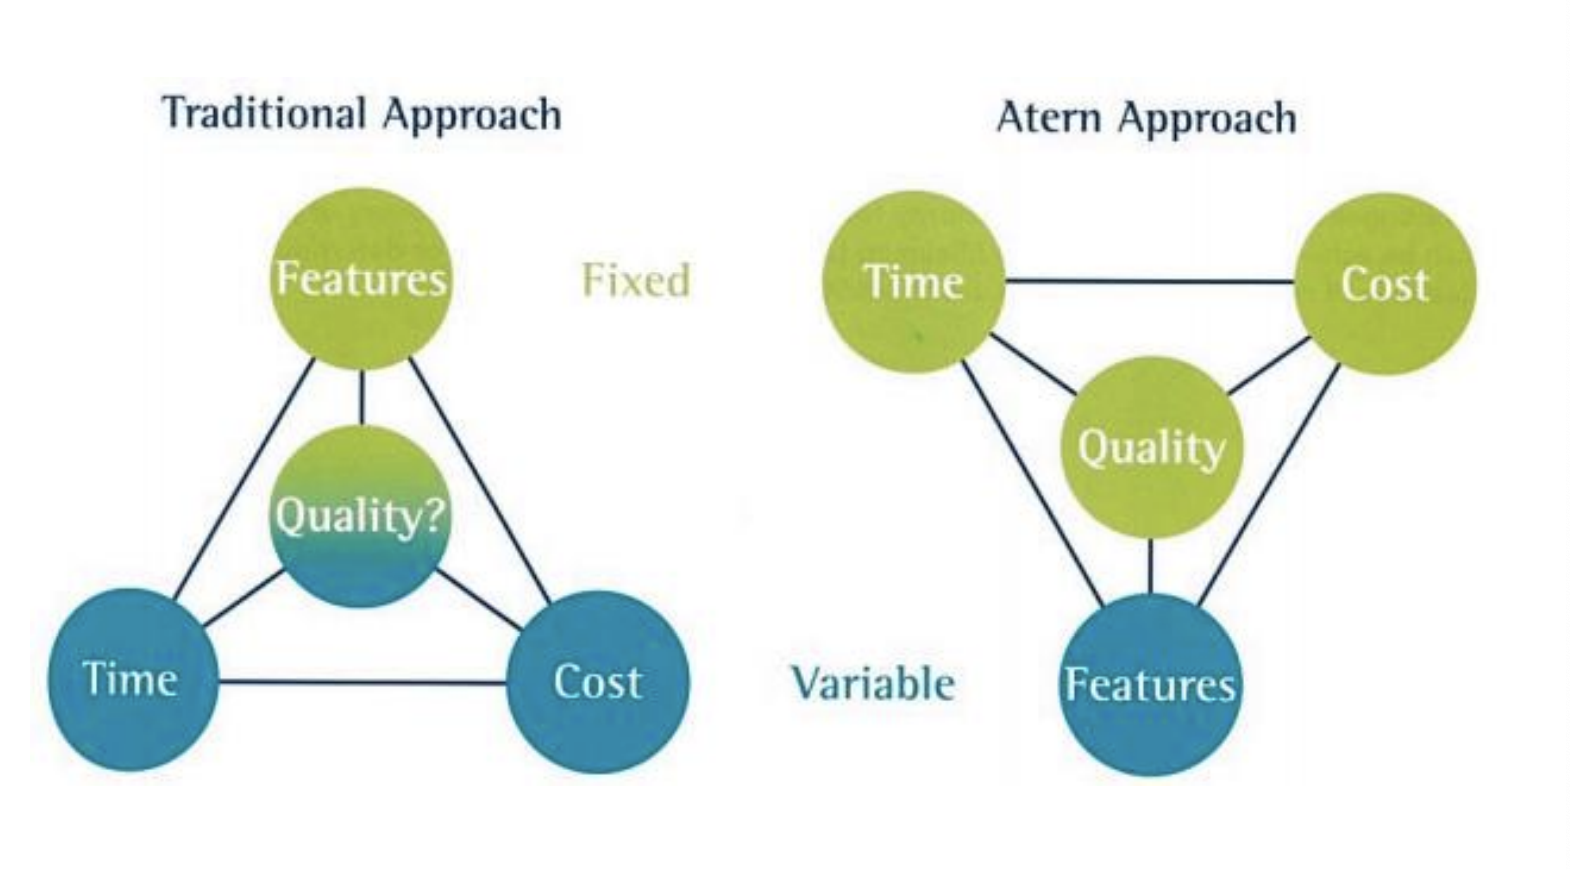
\includegraphics[width=\linewidth]{atern_approach.png}
    \end{figure}

    \textbf{PROCESS - PEOPLE - PRODUCTS - PRACTISES}
    \begin{itemize}
        \item Focus on the \textit{business need}
        \item Deliver \textit{on time}
        \item \textit{Collaborate}
        \item Never compromise \textit{quality}
        \item Build incrementally from \textit{firm foundations}
        \item Develop \textit{iteratively}
        \item \textit{Communicate continuously} and clearly
        \item Demonstrate \textit{control}
    \end{itemize}



    \subsubsection{Fazy projektu}
    \begin{figure}[H]
        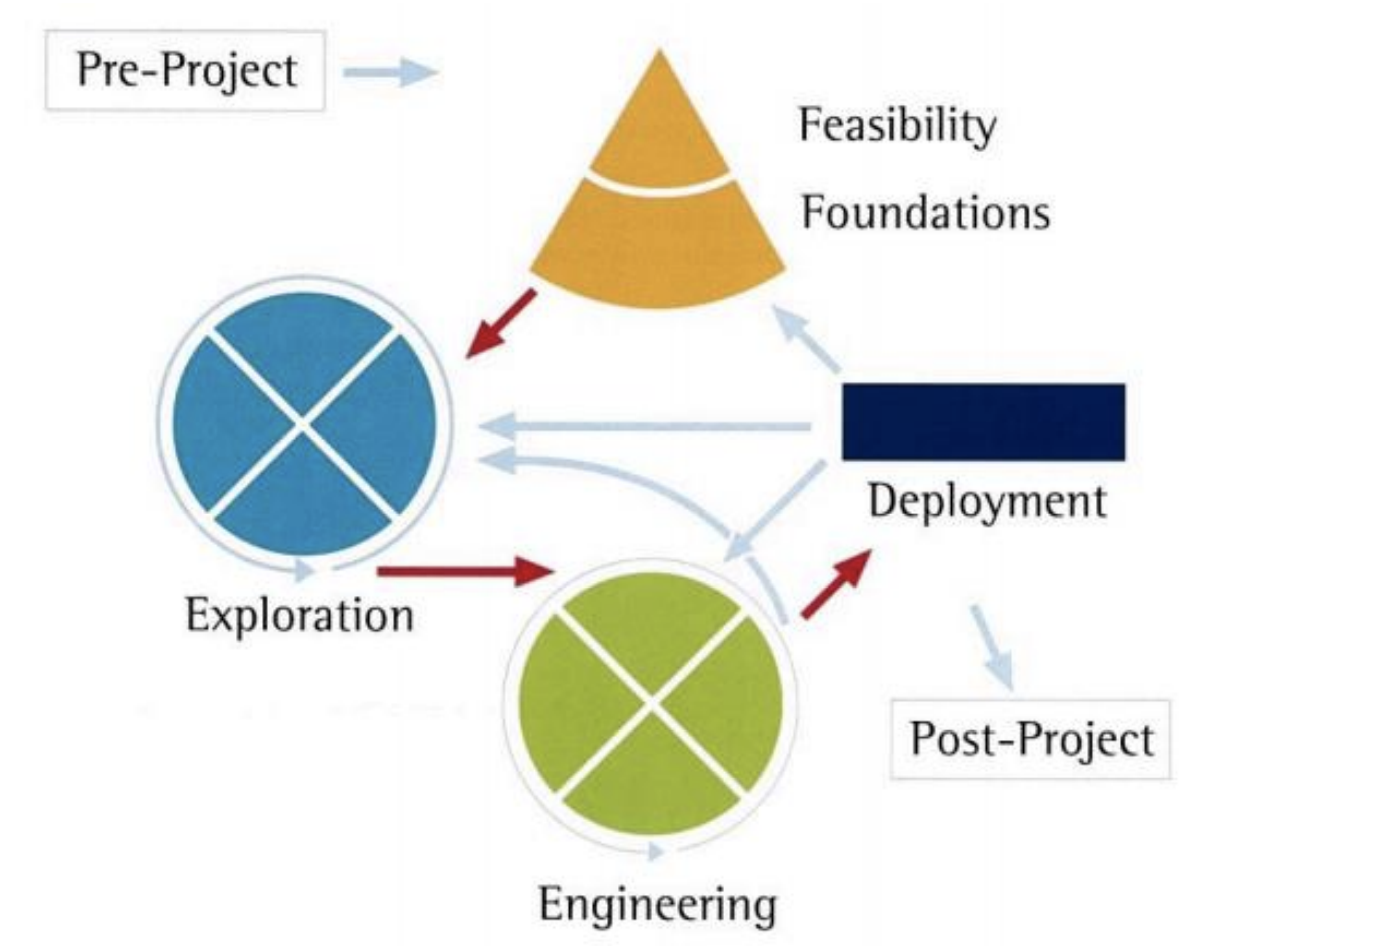
\includegraphics[width=\linewidth]{agile_fazy.png}
    \end{figure}

    \begin{itemize}
        \item \textbf{Pre-project}
        \begin{itemize}
            \item problem biznesowy; identyfikacja Business Sponsor i Business Visionary,
            \item zakres, plan i zasoby na fazę Feasibility.
        \end{itemize}
        \item \textbf{Feasibility}
        \begin{itemize}
            \item ustalić wykonalność rozwiązania problemu biznesowego,
            \item identyfikacja potencjalnych zysków; zarys możliwych podejść do rozwiązania,
            \item pierwsze estymaty czasowe i kosztowe.
        \end{itemize}
        \item \textbf{Foundation}
        \begin{itemize}
            \item wysoko poziomowe wymagania,
            \item identyfikacja wspieranych procesów biznesowych,
            \item podstawy architektury systemu; sposób zapewnienia wysokiej jakości.
        \end{itemize}
        \item \textbf{Exploration}
        \begin{itemize}
            \item uszczegóławianie wymagań; iteracyjnie działające rozwiązanie,
            \item zarys możliwych podejść do rozwiązania.
        \end{itemize}
        \item \textbf{Engineering}
        \begin{itemize}
            \item rozwijanie rozwiązania z fazy Exploration.
        \end{itemize}
        \item \textbf{Deployment}
        \begin{itemize}
            \item potwierdzenie wydajności rozwiązania,
            \item dostarczenie (iteracyjnie) rozwiązania,
            \item dostarczenie potrzebnej dokumentacji.
        \end{itemize}
    \end{itemize}

    \subsubsection{Role}
    \begin{itemize}
        \item \textbf{Business Sponsor}
        \begin{itemize}
            \item najwyższy rangą w projekcie; zapewnia finansowanie i zasoby,
            \item właściciel tzw. przypadku biznesowego.
        \end{itemize}
        \item \textbf{Business visionary}
        \begin{itemize}
            \item definiuje wizję projektu i komunikuje ją,
            \item ma zapewnić współprace na wszystkich poziomach projektu,
            \item wkład w najważniejsze wymagania; arbiter w przypadku sporów.
        \end{itemize}
        \item \textbf{Project manager}
        \begin{itemize}
            \item monitoruje postęp projektu; motywuje zespoły, zatrudnia specjalistów,
            \item wysoko poziomowe planowanie harmonogramu, zarządzanie ryzykiem w projekcie.
        \end{itemize}
        \item \textbf{Technical coordination}
        \begin{itemize}
            \item definiuje środowisko pracy,
            \item doradza w sprawach technicznych, pilnuje standardów,
            \item zajmuje się wymaganiami niefunkcjonalnymi.
        \end{itemize}
        \item \textbf{Team Leader}
        \begin{itemize}
            \item skupiony na zespole, pilnuje dostarczania poszczególnych komponentów na czas,
            \item raportuje postęp do PM, prowadzi spotkania zespołowe.
        \end{itemize}
        \item \textbf{Business Ambassador}
        \begin{itemize}
            \item rola biznesowa w zespole deweloperskim,
            \item dzieli się perspektywa biznesową z zespołem, dostarcza scenariusze biznesowe,
            \item tworzy dokumentacje użytkownika.
        \end{itemize}
        \item \textbf{Business Analyst}
        \begin{itemize}
            \item komunikacja między biznesem a zespołem deweloperskim,
            \item dystrybucja i wstępna akceptacja dokumentów biznesowych.
        \end{itemize}
        \item \textbf{Solution Developer}
        \begin{itemize}
            \item skupiony na dostarczeniu rozwiązania,
            \item modele potrzebne do dostarczenia rozwiązania, dokumentacja.
        \end{itemize}
        \item \textbf{Solution Tester}
        \begin{itemize}
            \item definiuje scenariusze testowe, test casy,
            \item komunikuje wyniki testów do TL, pracuje z BAs nad testami akceptacyjnymi.
        \end{itemize}
        \item
    \end{itemize}

    \subsubsection{Produkty}

    Levels of priority - \textbf{MoSCoW}
    \begin{itemize}
        \item \textbf{M}ust Have
        \item \textbf{S}hould Have
        \item \textbf{C}ould Have
        \item \textbf{W}on’t Have this time
    \end{itemize}

    Fazy \textbf{TIMEBOX}u:
    \begin{itemize}
        \item \textbf{Kick-off} – krótka sesja, która ma pomoc zrozumieniu celu timeboxa,
        \item \textbf{Investigation} – szczegóły wszystkich produktów, które mamy wykonać,
        \item \textbf{Refinement} – kodowanie i testowanie,
        \item \textbf{Consolidation} – spinanie całości.
    \end{itemize}

    \textbf{Iterative development}:
    \begin{itemize}
        \item \textbf{Identify}: zespół definiuje cel
        \item \textbf{Plan}: kto powinien zrobić co
        \item \textbf{Evolve}: wykonywanie
        zaplanowanych czynności
        \item \textbf{Review}: sprawdzanie rezultatów
    \end{itemize}


    \begin{figure}[H]
        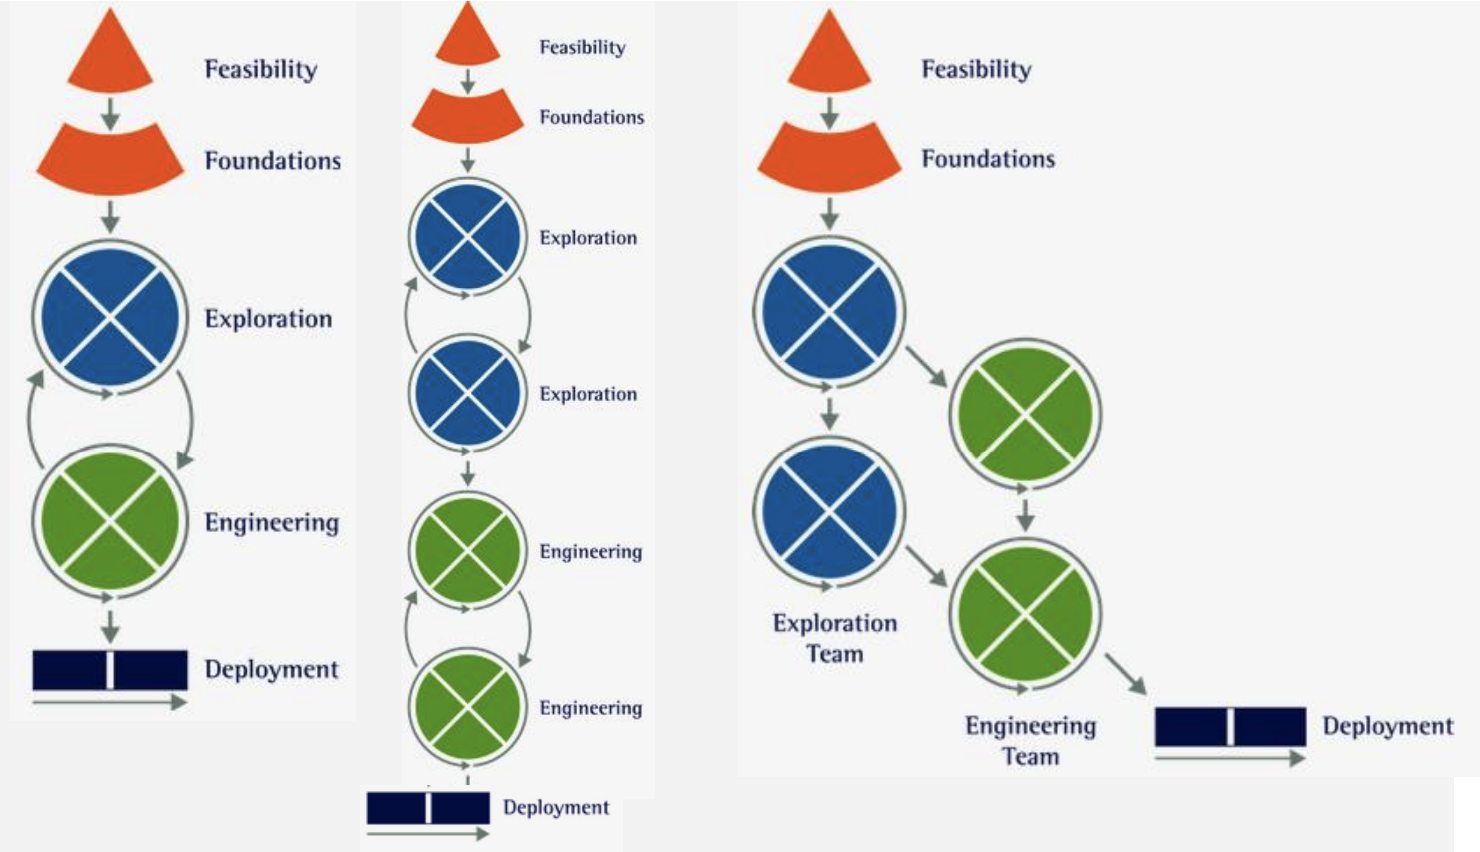
\includegraphics[width=\linewidth]{agile_iterations.png}
    \end{figure}


    \subsection{AUP - Agile Unified Process}

    \begin{itemize}
        \item uproszczona wersja Rational Unified Process,
        \item stosuje zwinne techniki takie jak TDD, refactoring,
        \item \textbf{seryjny w dużej skali, iteracyjny w małej}.
    \end{itemize}


    \begin{figure}[H]
        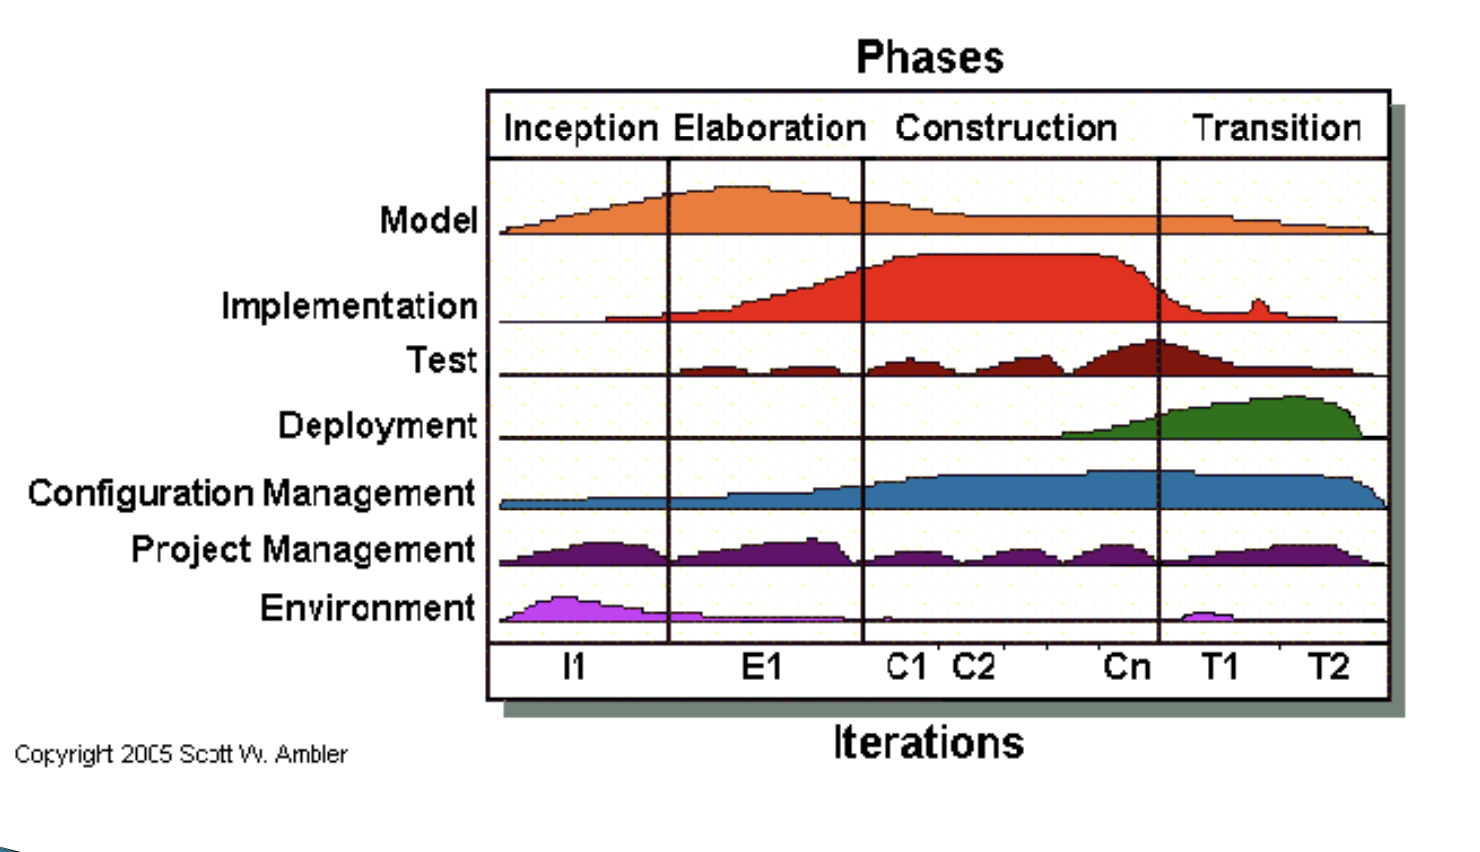
\includegraphics[width=\linewidth]{aup_phases.png}
    \end{figure}


    \textbf{Zasady AUP}
    \begin{itemize}
        \item twój zespół wie, co robi;
        \item prostota;
        \item zwinność;
        \item skupienie się na istotnych aktywnościach;
        \item niezależność od narzędzi;
        \item możliwość adaptacji.
    \end{itemize}


    \subsection{KANBAN}
    \begin{itemize}
        \item jedna z podstaw systemów produkcyjnych Toyoty  i pochodnych, opartych o zasadę pull.
        \item \textbf{System pull} (w odróżnieniu od systemów push), sterowany
        jest przez \textbf{składane przez odbiorcę zamówienie}, a nie ogólny, arbitralny plan produkcji. Za pomocą
        techniki kanban zapewnia się \textit{ciągły przepływ produktu przez system produkcyjny}.
        \item odnosi się do \textbf{etapowości procesu wytwarzania
        oprogramowania} (skojarzenia z procesami kaskadowymi). Zawsze występują jednak przynajmniej trzy stany pracy — do
        zrobienia, w trakcie, gotowe.
    \end{itemize}

    \textbf{Sześć reguł kanbana}:
    \begin{itemize}
        \item odbiorca przetwarza dokładnie tyle elementów, ile opisane
        jest na karcie kanban;
        \item dostawca wytwarza dokładnie tyle elementów, ile opisane jest
        na karcie kanban;
        \item żaden element nie jest wytwarzany lub przekazywany
        pomiędzy stanowiskami bez karty kanban;
        \item karta kanban musi towarzyszyć każdemu elementowi czy
        półproduktowi przetwarzanemu w ramach systemu;
        \item elementy wadliwe lub występujące w niewłaściwych ilościach,
        nigdy nie są przekazywane w dół procesu;
        \item limity obowiązujące na każdym z etapów (fizyczna ilość kart
        kanban) są stopniowo obniżane aby redukować zapasy i
        odkrywać nieefektywności procesów produkcji, dążąc do ich
        doskonalenia.
    \end{itemize}

    Kanban vs Scrum
    \begin{figure}[H]
        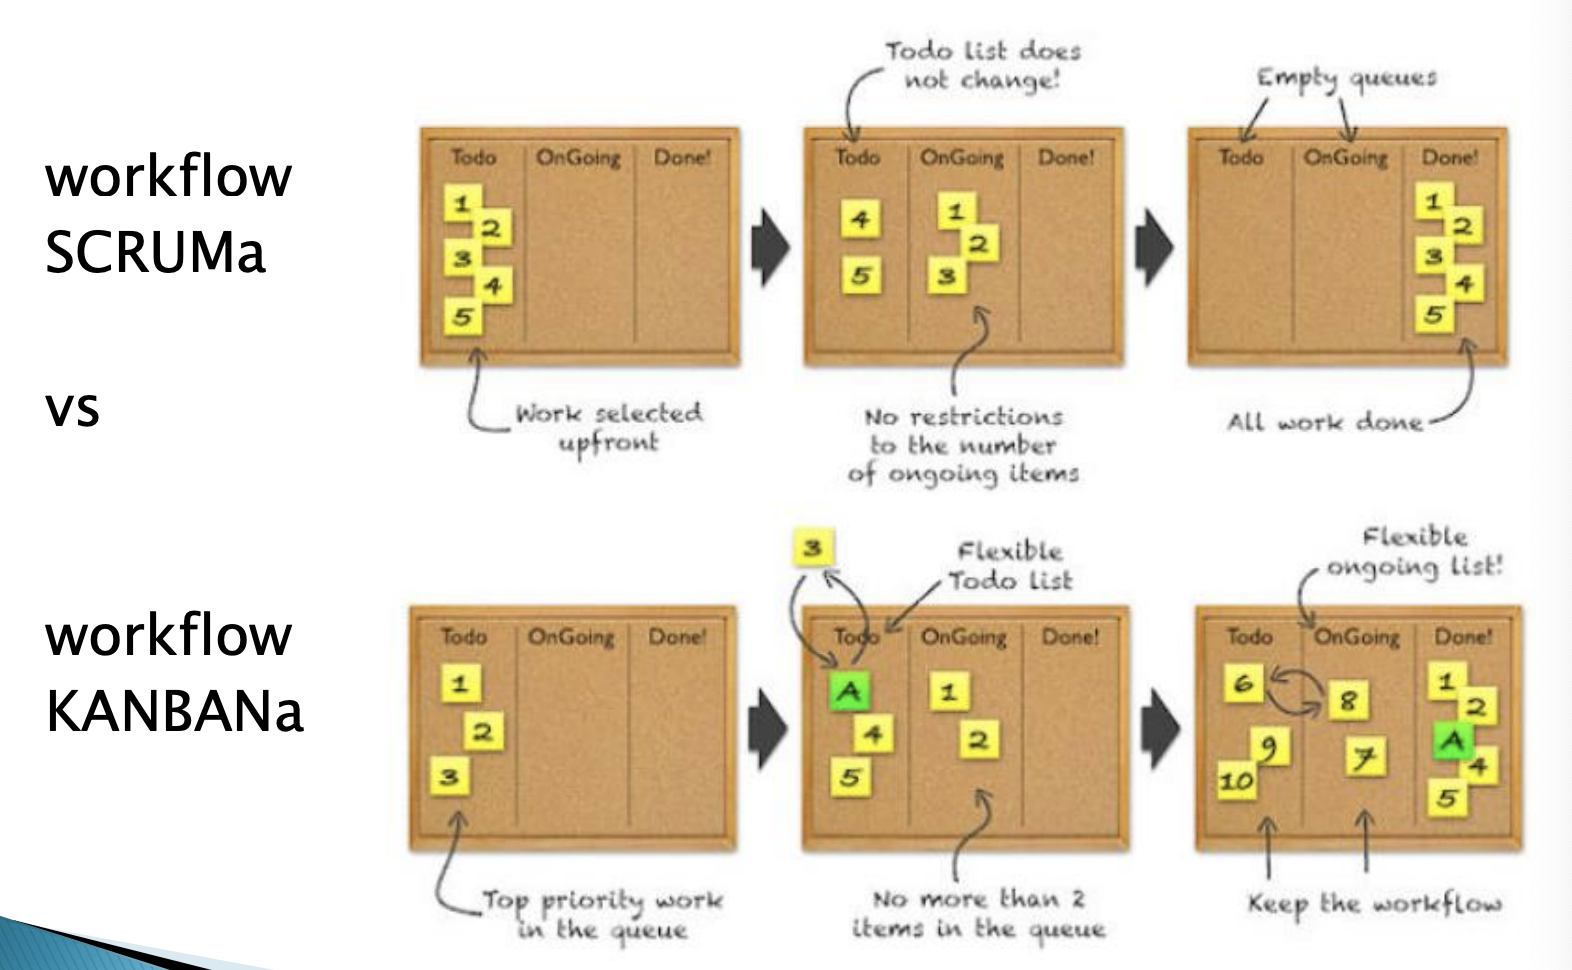
\includegraphics[width=\linewidth]{kanban_vs_scrum.png}
    \end{figure}
    \begin{figure}[H]
        \includegraphics[width=\linewidth]{kanban_vs_scrum2.png}
    \end{figure}
    \begin{figure}[H]
        \includegraphics[width=\linewidth]{kanban_vs_scrum3.png}
    \end{figure}
    \begin{figure}[H]
        \includegraphics[width=\linewidth]{kanban_vs_scrum4.png}
    \end{figure}

    \begin{figure}[H]
        \includegraphics[width=\linewidth]{kanban_vs_scrum5.png}
    \end{figure}

    \subsection{SCRUM + KANBAN = SCRUM-BAN}
    Kiedy używać Scrum-bana?
    \begin{itemize}
        \item W projektach typu maintenance
        \item W projektach typu helpdesk
        \item W projektach z często dorzucanymi User stories
        lub często zgłaszanymi bledami
    \end{itemize}

    \begin{figure}[H]
        \includegraphics[width=\linewidth]{scrum_vs_scrumban.png}
    \end{figure}

    \section{Wymagania}
    \begin{itemize}
        \item Wymagania to \textbf{opis funkcji} (usług) i ograniczeń dla systemu.
        \item Wymagania nie opisują jak system ma działać, a \textbf{co ma
        wykonywać}.
        \item Definiowane na \textbf{wczesnych etapach rozwoju} systemu jako specyfikacja tego, co ma być
        implementowane.
        \item Inżynieria wymagań to proces pozyskiwania, analizowania, dokumentowania oraz weryfikowania
        wymagań dla projektowanego systemu.

    \end{itemize}

    \subsection{Klasyfikacja wymagań}
    \begin{itemize}
        \item \textbf{Funkcjonalne} - czynność, zadanie.
        \item \textbf{Pozafunkcjonalne} - technikalia mierzone metrykami.
    \end{itemize}

    \textbf{Klasyfikacja wymagań - FURPS} - \textbf{F}unctionality, \textbf{U}sability, \textbf{R}eliability,
   \textbf{P}erformance, \textbf{S}ecurity.

    \subsubsection{Wymagania funkcjonalne}
    „System powinien\dots”
    \begin{itemize}
        \item \textbf{Zalety}: łatwość spisywania,
        \item \textbf{Wady}: słaba czytelność, trudne sprawdzanie kompletności i spójności.
    \end{itemize}

\hfill \\
    \textbf{Przypadki użycia}
    \begin{itemize}
        \item \textbf{Zalety}: łatwość spisywania, czytelność, łatwość zrozumienia i wyobrażenia sobie
        przyszłego systemu.
        \item forma ustrukturalizowana.
    \end{itemize}

    \textbf{Historyjki użytkownika} - Who? What? Why?\\
    Cecha \textbf{INVEST} \textbf{I}ndependent (zależności powodują problem z estymacją), \textbf{N}egotiable, \textbf{V}aluable, \textbf{E}stimable, \textbf{S}mall (jeden sprint), \textbf{T}estable.


    \subsubsection{Wymagania pozafunkcjonalne}
    Ograniczenia usług lub funkcji, np. ograniczenia czasowe, ograniczenia procesu rozwoju oprogramowania, standardy.
    Każda cecha to \textbf{zbiór atrybutów}.


    \begin{itemize}
        \item Stanowią \textbf{niezbędne uzupełnienie wymagan funkcjonalnych} dla oprogramowania,
        \item Problemy z oprogramowaniem wskazują na silną potrzebę precyzyjnego definiowania atrybutów
        (charakterystyk) dla tworzonych produktów programistycznych.
    \end{itemize}

    \begin{itemize}
        \item \textbf{Niezawodność} - zdolność oprogramowania do spełnienia i utrzymania
        określonych wymagań stabilności działania, przy spełnieniu określonych
        warunków oraz w ścile określonych ramach czasowych.
        \begin{itemize}
            \item Dojrzałość
            \item Odporność na błędy
            \item Zdolność do odtworzenia
        \end{itemize}
        \item \textbf{Wydajność} - opisuje powiązania miedzy poziomem wydajności oprogramowania, a
        wykorzystywanymi zasobami przy spełnieniu określonych warunków.
        \begin{itemize}
            \item Wykorzystanie czasu
            \item Wykorzystanie zasobów
        \end{itemize}
        \item \textbf{Użyteczność} - opisuje nakład pracy niezbędny do swobodnego posługiwania się oprogramowaniem.
        \begin{itemize}
            \item Łatwość zrozumienia
            \item Łatwość nauki
            \item Operatywność
        \end{itemize}
        \item \textbf{Łatwość konserwacji} - opisuje nakład pracy niezbędny do wprowadzenia zmian do oprogramowania.
        \begin{itemize}
            \item Łatwość analizy
            \item Łatwość wprowadzania zmian
            \item Stabilność
            \item Łatwość testowania
        \end{itemize}
        \item \textbf{Przenośność} - opisuje zdolność oprogramowania do przenoszenia między różnymi środowiskami/platformami.
        \begin{itemize}
            \item Łatwość adaptacji
            \item Zgodność
            \item Łatwość instalacji
            \item Łatwość zastąpienia
        \end{itemize}
    \end{itemize}


    \subsection{Analiza wymagań/analiza obiektowa}
    \begin{itemize}
        \item Celem jest stworzenie modelu systemu, zwanego \textbf{modelem analitycznym}.
        \item Wysiłek uczestników projektu skupia się na strukturalizowaniu i formalizowaniu zabranych
        wcześniej wymagań.
    \end{itemize}

    \textbf{Definicje}
    \begin{itemize}
        \item \textbf{Model analityczny} – reprezentuje tworzony system z perspektywy użytkownika; opis co system powinien robić.
        \item \textbf{Analityczny model obiektowy} – odzwierciedla indywidualne koncepcje korzystania z systemu, ich właściwości i relacje między nimi (diagramy klas).
        \item \textbf{Model dynamiczny} - koncentruje się na zachowaniu systemu(diagramy sekwencji i stanów).
        \item \textbf{Obiekty encji} – reprezentują trwałą informację potwarzaną przez system.
        \item \textbf{Obiekty brzegowe} – odzwierciedlają interakcje między aktorami a systemem.
        \item \textbf{Obiekty sterujące} – odpowiedzialne są za realizację przypadków użycia.
        \item \textbf{Relacja dziedziczenia} umożliwia hierarchiczne organizowanie koncepcji.
        \item \textbf{Generalizowanie} - aktywność identyfikowania abstrakcyjnych koncepcji na podstawie przykładów i konkretyzacji.
        \item \textbf{Specjalizowanie} - aktywność odwrotna, czyli identyfikowanie koncepcji bardziej specyficznych na podstawie koncepcji wysokopoziomowej.
    \end{itemize}

    \begin{figure}[h]
        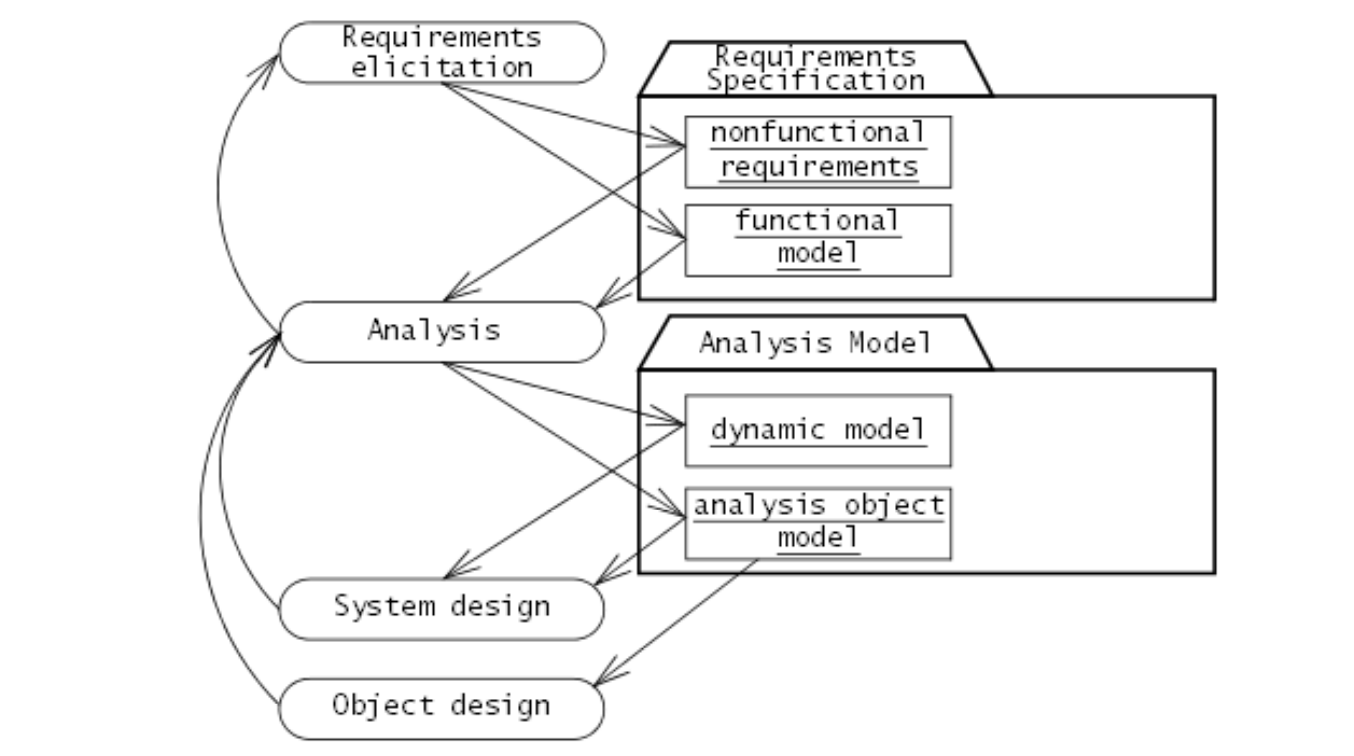
\includegraphics[width=\linewidth]{analiza_wymagan.png}
    \end{figure}

    \section{Projektowanie systemu}
    \textbf{Transformowanie modelu analitycznego w model projektu systemu.}

    Etapy projektowania systemu:
    \begin{itemize}
        \item rozpoznawanie celów projektowych,
        \item projektowanie wstępnych dekompozycji,
        \item doskonalenie dekompozycji stosownie do celów projektowych.
    \end{itemize}

    \begin{figure}[H]
        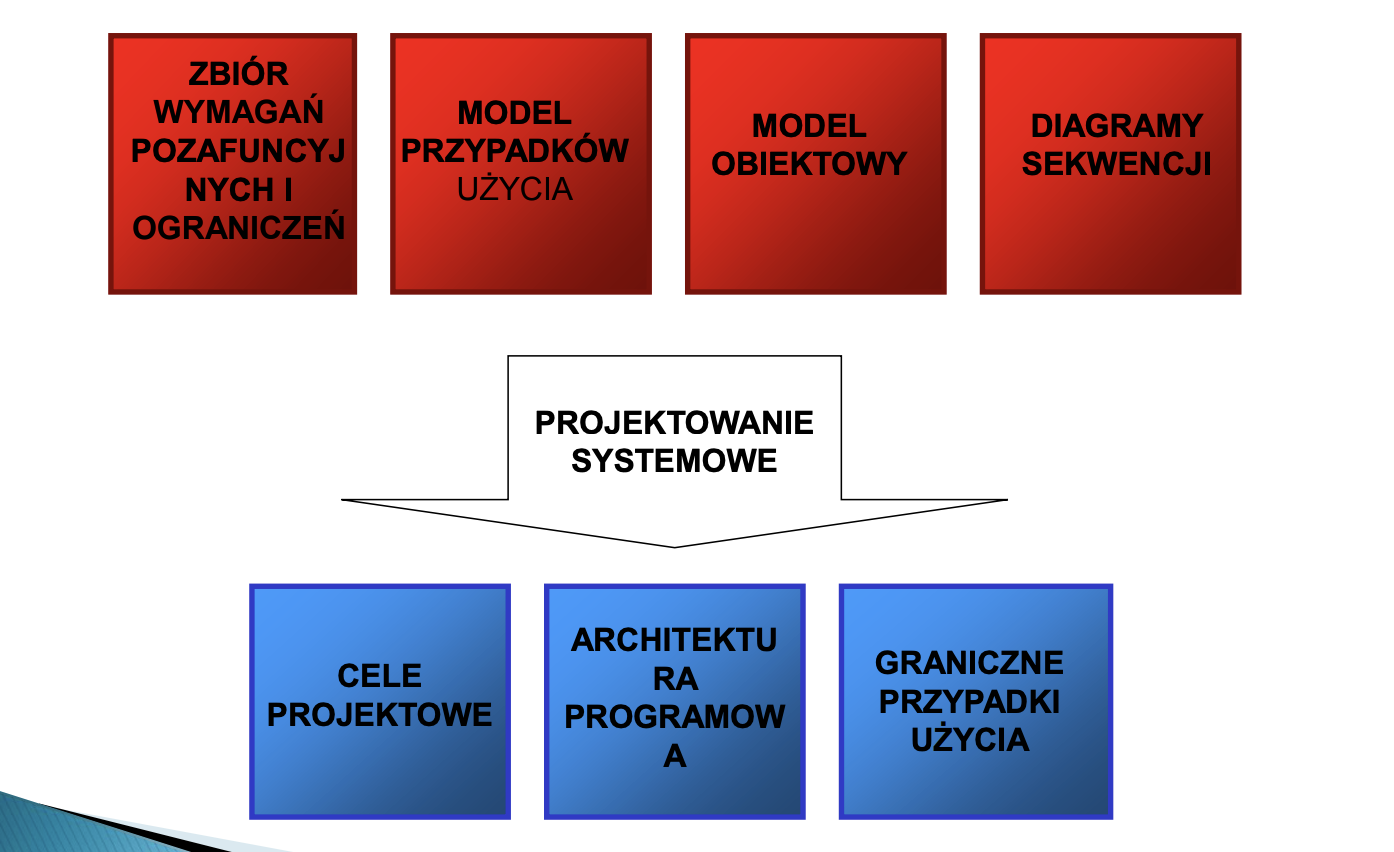
\includegraphics[width=\linewidth]{projekt_systemu.png}
    \end{figure}

    \subsection{Podstawowe pojęcia i koncepcje.}
    \begin{itemize}
        \item \textbf{Podsystem} - wymienna część systemu, posiadającą dobrze zdefiniowane interfejsy i
        hermetyzującą stan oraz zachowanie składających się na nią klas.
        \item Dwa główne typy komponentów: \textbf{logiczny i fizyczny}.
        \item \textbf{Usługa} jest zbiorem powiązanych operacji podporządkowanych realizacji wspólnego
        celu.
        \item \textbf{Sprzężeniem} w zbiorze podsystemów nazywamy stopień ich \textbf{wzajemnego uzależnienia}. (MINIMALIZACJA)
        \item \textbf{Spoistość} podsystemu jest miara \textbf{uzależnienia jego własnych klas}. (MAKSYMALIZACJA)
        \item \textbf{Warstwa} - zgrupowanie podsystemów oferujących powiązane usługi.
        \item Efektem \textbf{dekompozycji hierarchicznej} jest uporządkowany zbiór warstw.
        \item \textbf{Architektury warstwowa}: otwarta i zamknięta (np ISO/OSI, TCP/IP).
    \end{itemize}


    \subsection{Wzorce architektoniczne - poziom integracji komponentów}

    \subsubsection{MVC: model-widok-kontroler}
    Model zawiera korowa funkcjonalność. Widoki wyświetlają funkcjonalności. Kontroler obsługuje żądanie użytkownika. Kontroler z widokami tworzą UI aplikacji.

    Zastosowania: Smalltalk, Java/Swing.

    \begin{figure}[H]
        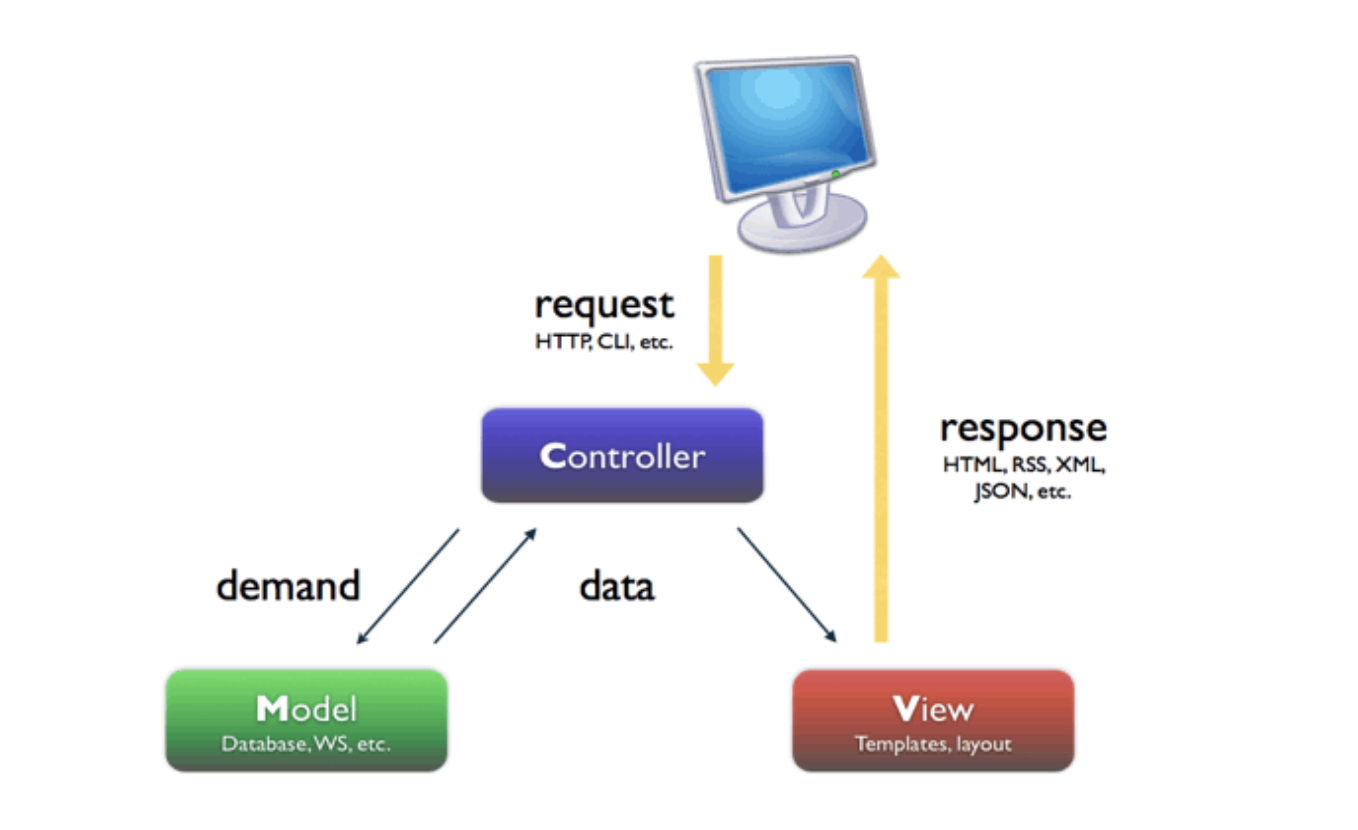
\includegraphics[width=.5\linewidth]{mvc.png}
        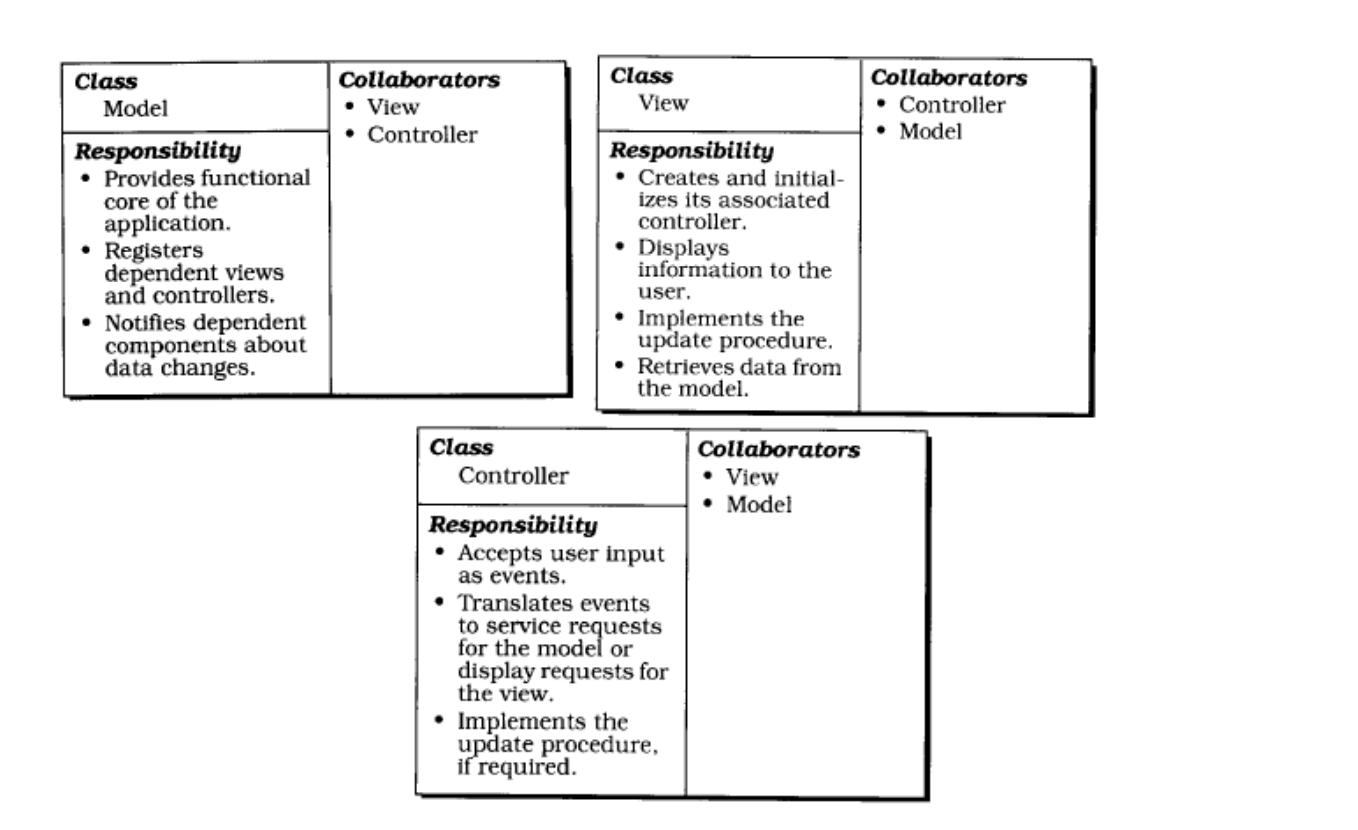
\includegraphics[width=.5\linewidth]{mvc-struktura.png}
    \end{figure}



    \subsubsection{PAC: prezentacja-abstrakcja-kontrola}
    Hierarchie kooperujących agentów,podzielonych na trzy komponenty: prezentacji, abstrakcji kontroli.

    Zastosowania: Network Trafic Management (gathering traffic datha, displaying various user-configurable
    views of the whole network).

    \begin{figure}[h]
        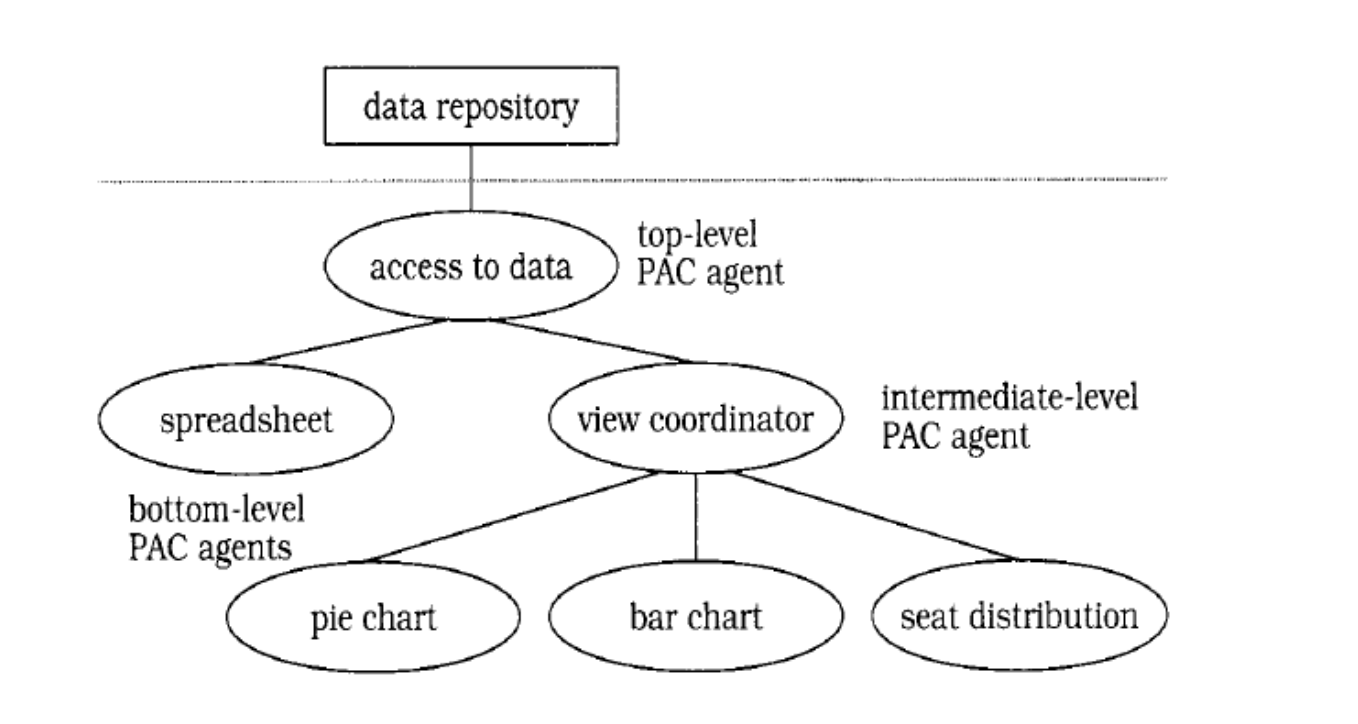
\includegraphics[width=.5\linewidth]{pac.png}
        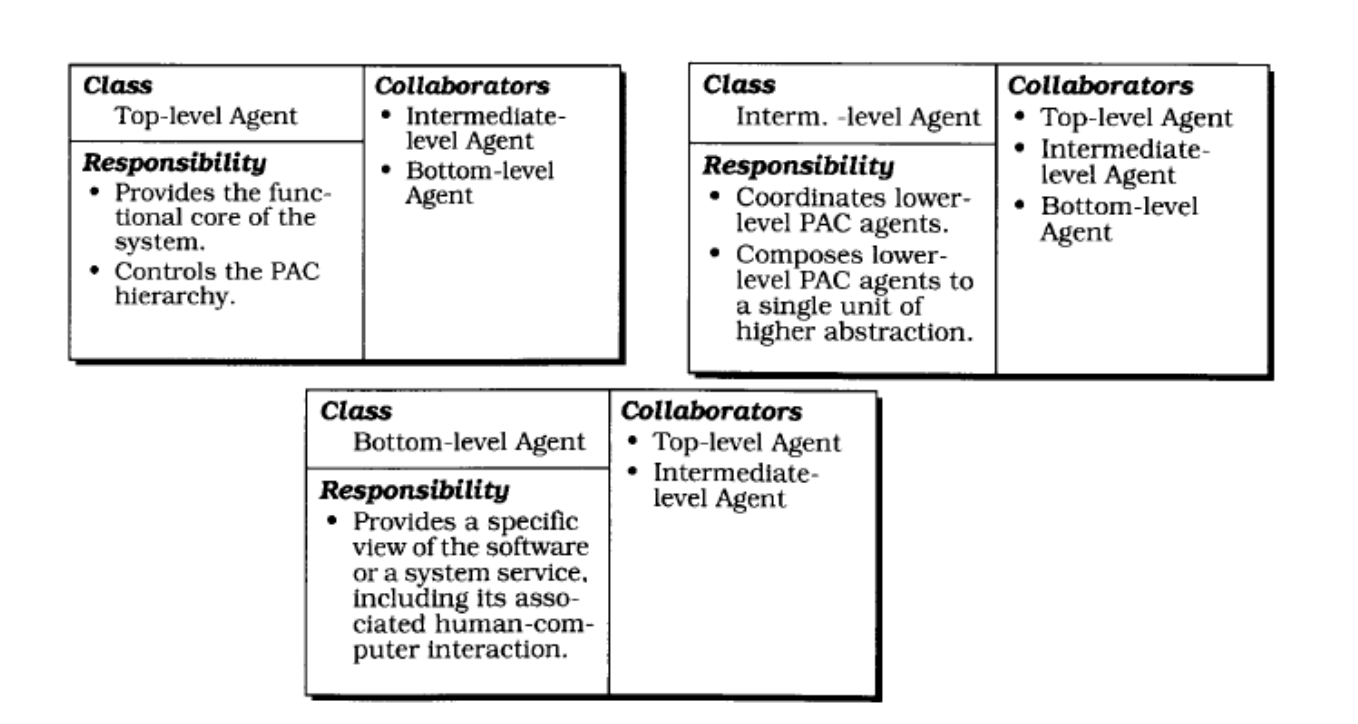
\includegraphics[width=.5\linewidth]{pac-struktura.png}
    \end{figure}



    \subsubsection{Architektura filtry i potoki}

    Pozwala na uporządkowanie systemu, który przetwarza strumienie danych. Każdy krok przetwarzania jest zamknięty w filtrze.
    Dane są przesyłane za pomocą potoków. Każdy z podsystemów realizuje przetwarzanie danych otrzymanych od innych podsystemów.

    Zastosowania: Unix, WEB, Servlet, Numerical Analysis (filters and data extractions).

    \begin{figure}[h]
        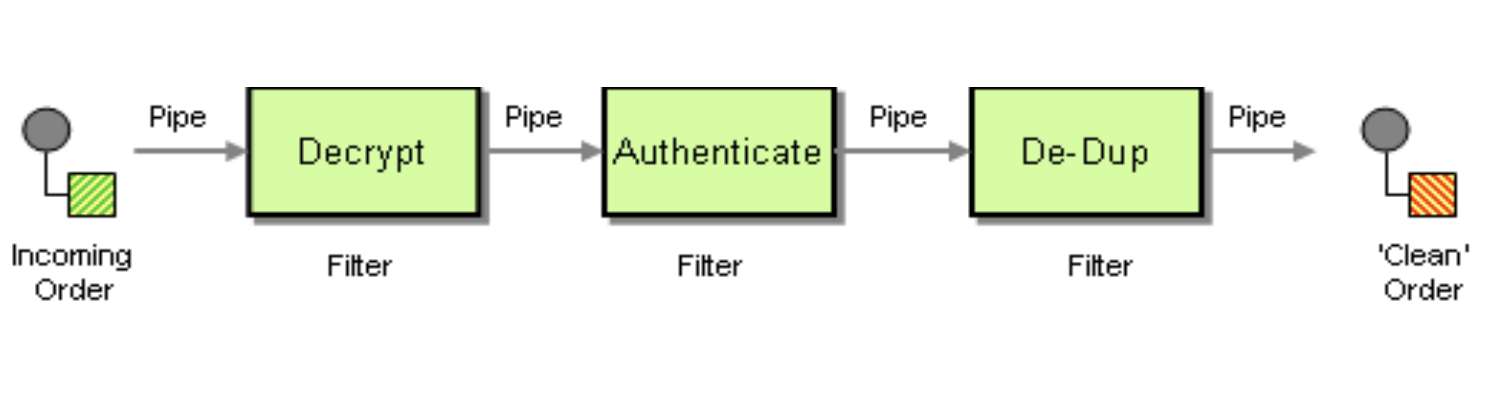
\includegraphics[width=.5\linewidth]{fip.png}
        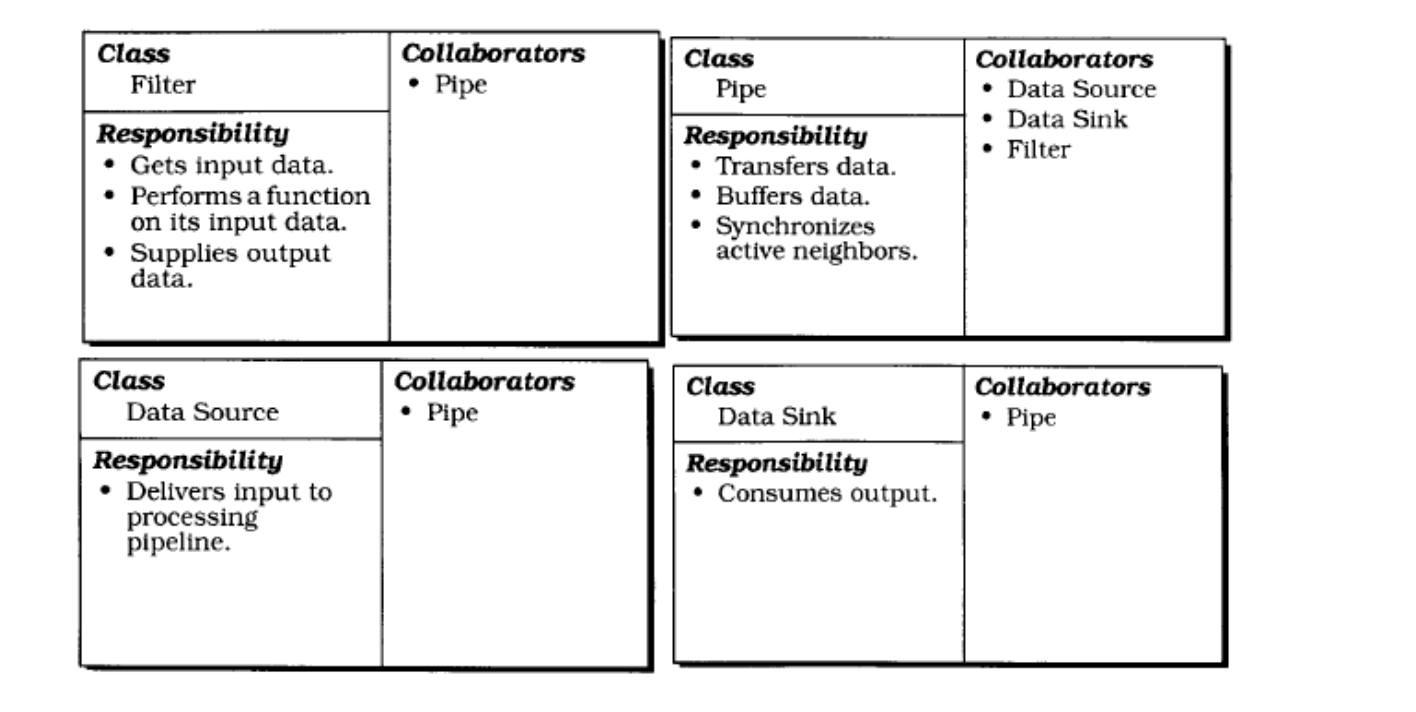
\includegraphics[width=.5\linewidth]{fip_struktura.png}
    \end{figure}




    \subsubsection{Tablica(blackboard)}
    Użyteczna w systemach, gdzie nie są znane deterministyczne rozwiązania danego problemu. W przypadku tablicy kilka wyspecjalizowanych
    systemów łączy swoja wiedze w taki sposób, żeby stworzyć częściowe lub przybliżone rozwiązanie problemu.

    Zastosowania: working memory, repository data.

    \begin{figure}[h]
        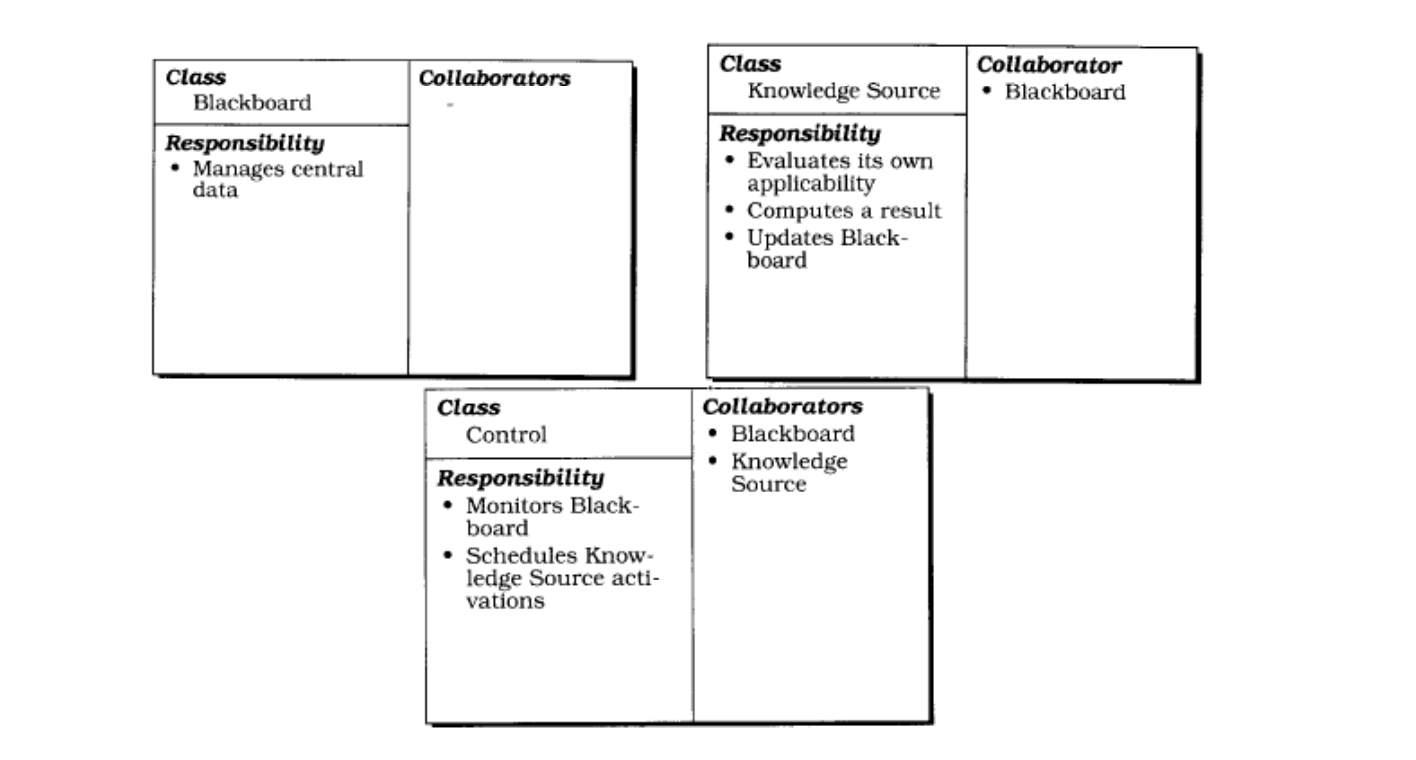
\includegraphics[width=.5\linewidth]{tablica.png}
    \end{figure}



    \subsubsection{Broker}
    Pozwala na uporządkowanie rozproszonych systemów podzielonych na komponenty współpracujące ze sobą za pomocą zdalnego wywoływania
    serwisu. Komponent brokera odpowiedzialny jest za koordynację komunikacji.

    \begin{figure}[h]
        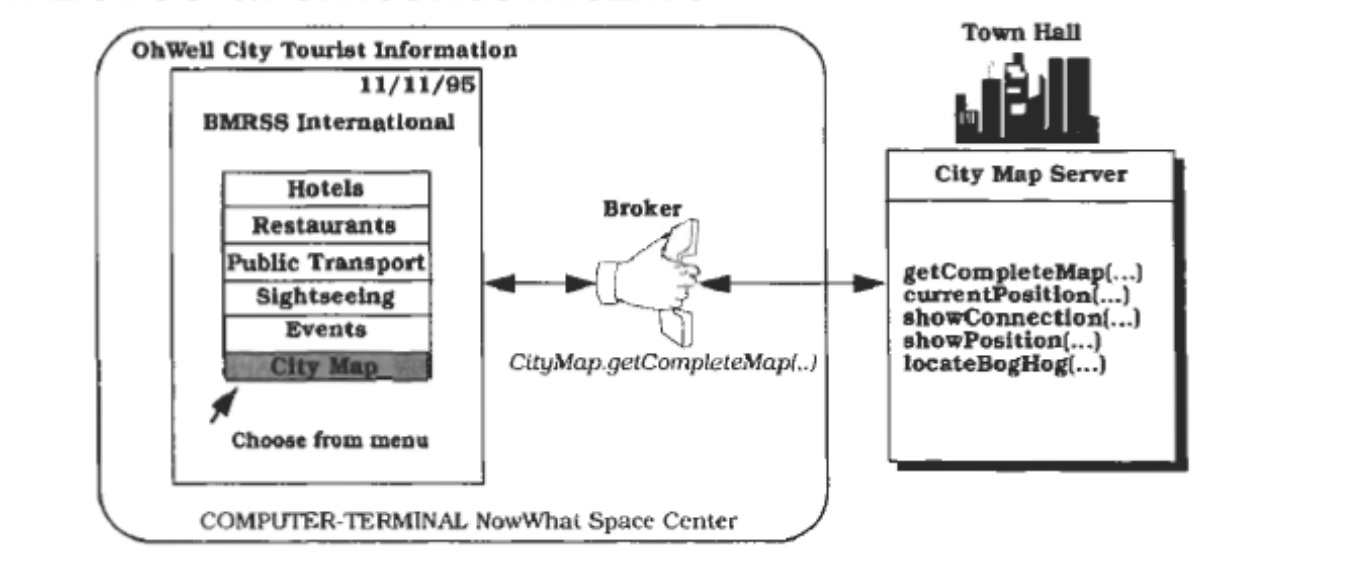
\includegraphics[width=.5\linewidth]{broker.png}
        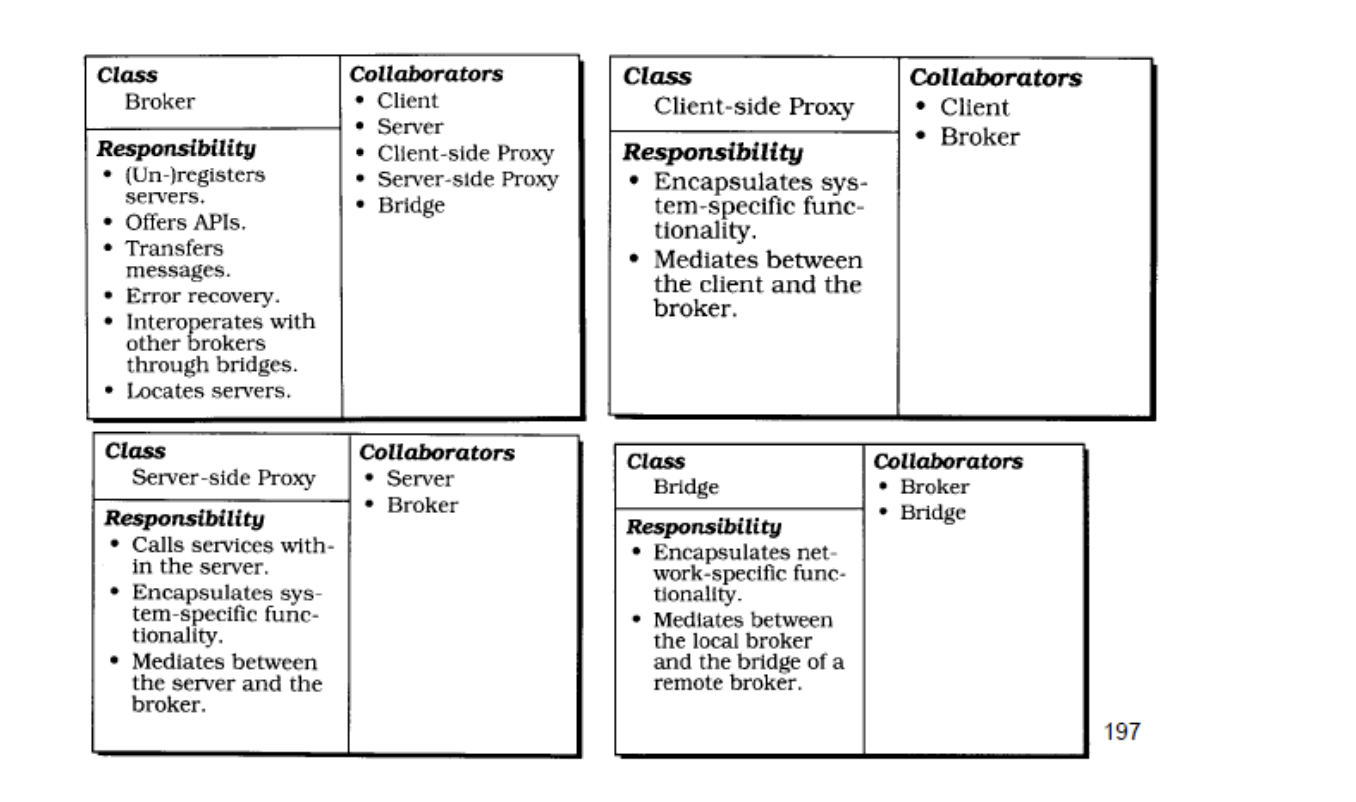
\includegraphics[width=.5\linewidth]{broker_struktura.png}
    \end{figure}

    \subsubsection{Reflection}
    Dostarcza mechanizm pozwalający na dynamiczną zmianę zachowania i struktury systemu.
    \begin{figure}[h]
        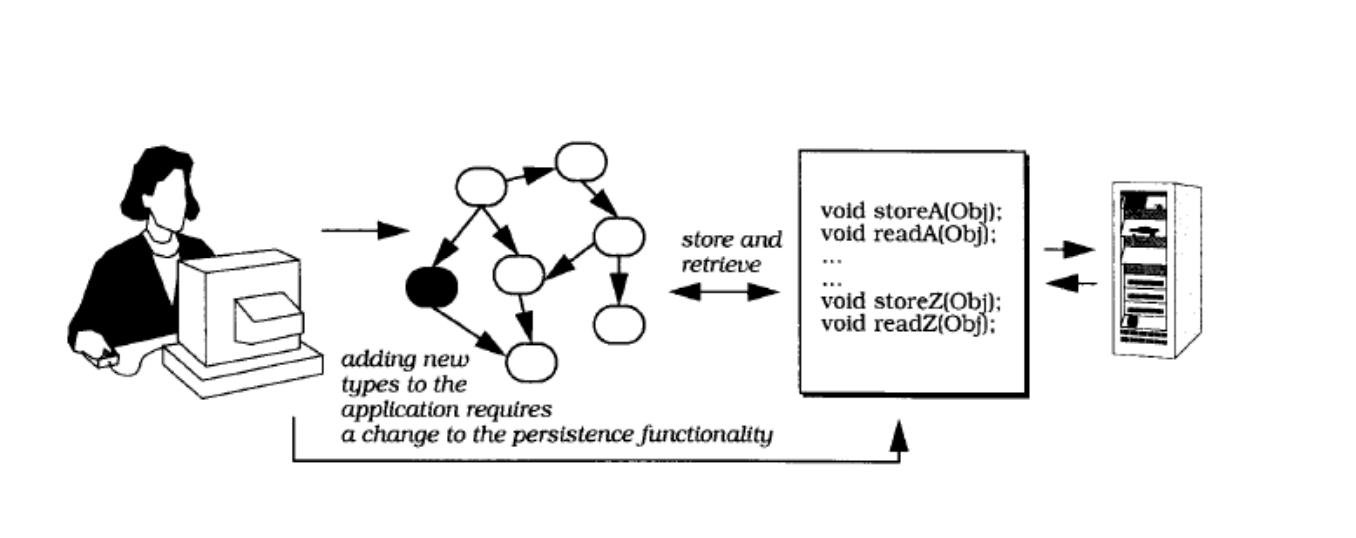
\includegraphics[width=.5\linewidth]{ref.png}
        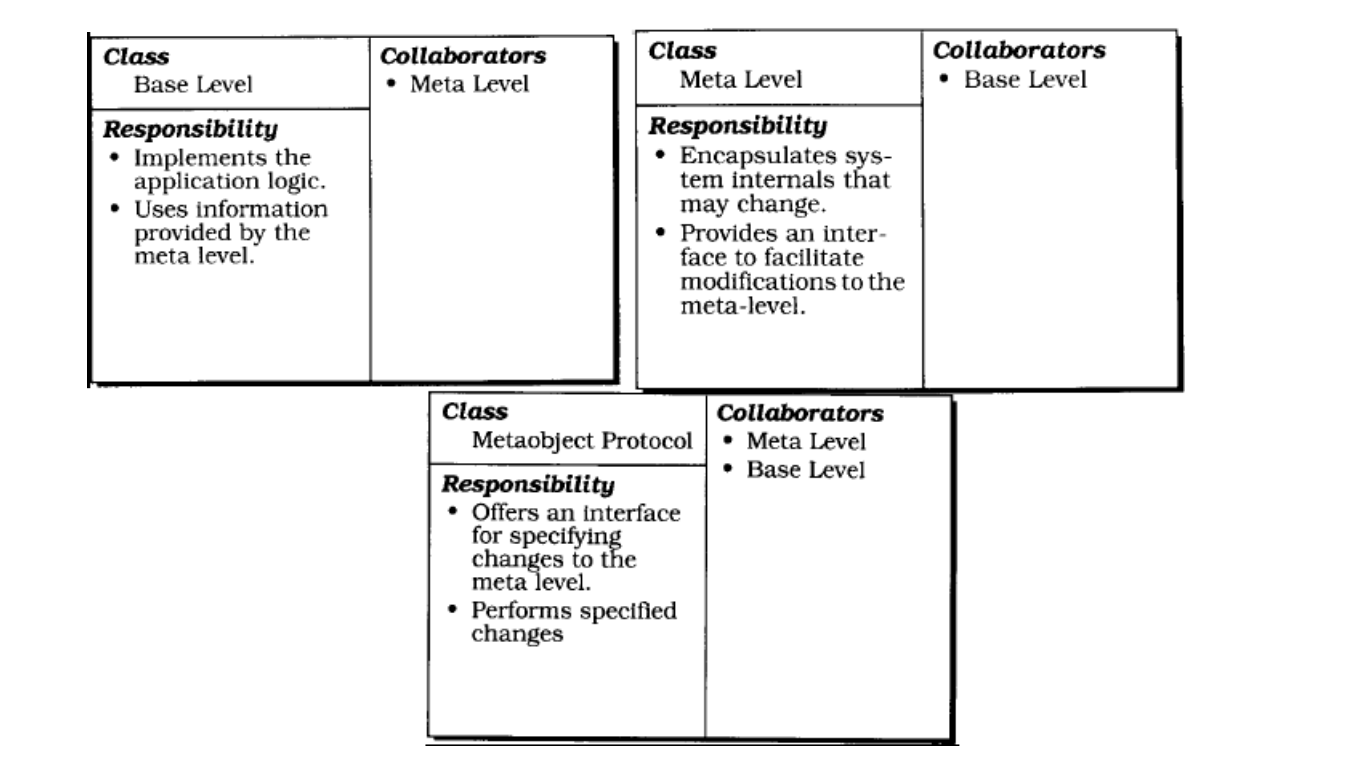
\includegraphics[width=.5\linewidth]{ref_struktura.png}
    \end{figure}

    Zastosowania: WWW.

    \subsubsection{Sieciowe}
    \begin{itemize}
        \item \textbf{Architektura klient-serwer} - podział systemu na dostawce usług (serwer) oraz ich odbiorców (klientów).
        \item \textbf{Architektura peer-to-peer} - każdy z podsystemów może spełniać obie funkcje (klient/serwer).

    \end{itemize}

    \subsubsection{Wzorce architektoniczne - wady}
    \begin{itemize}
        \item Patterns do not lead to direct code reuse.
        \item Individual Patterns are deceptively simple.
        \item Composition of different patterns can be very complex.
        \item Teams may suffer from pattern overload.
        \item Patterns are validated by experience and discussion
        rather than by automated testing.
        \item Integrating patterns into a software development
        process is a human-intensive activity.
    \end{itemize}


    \section{Projektowanie obiektów}
    Ma na celu \textbf{wypełnienie luki między obiektami dziedziny aplikacyjnej a komponentami} wybranymi na etapie projektowania systemu.


    \begin{figure}[h]
        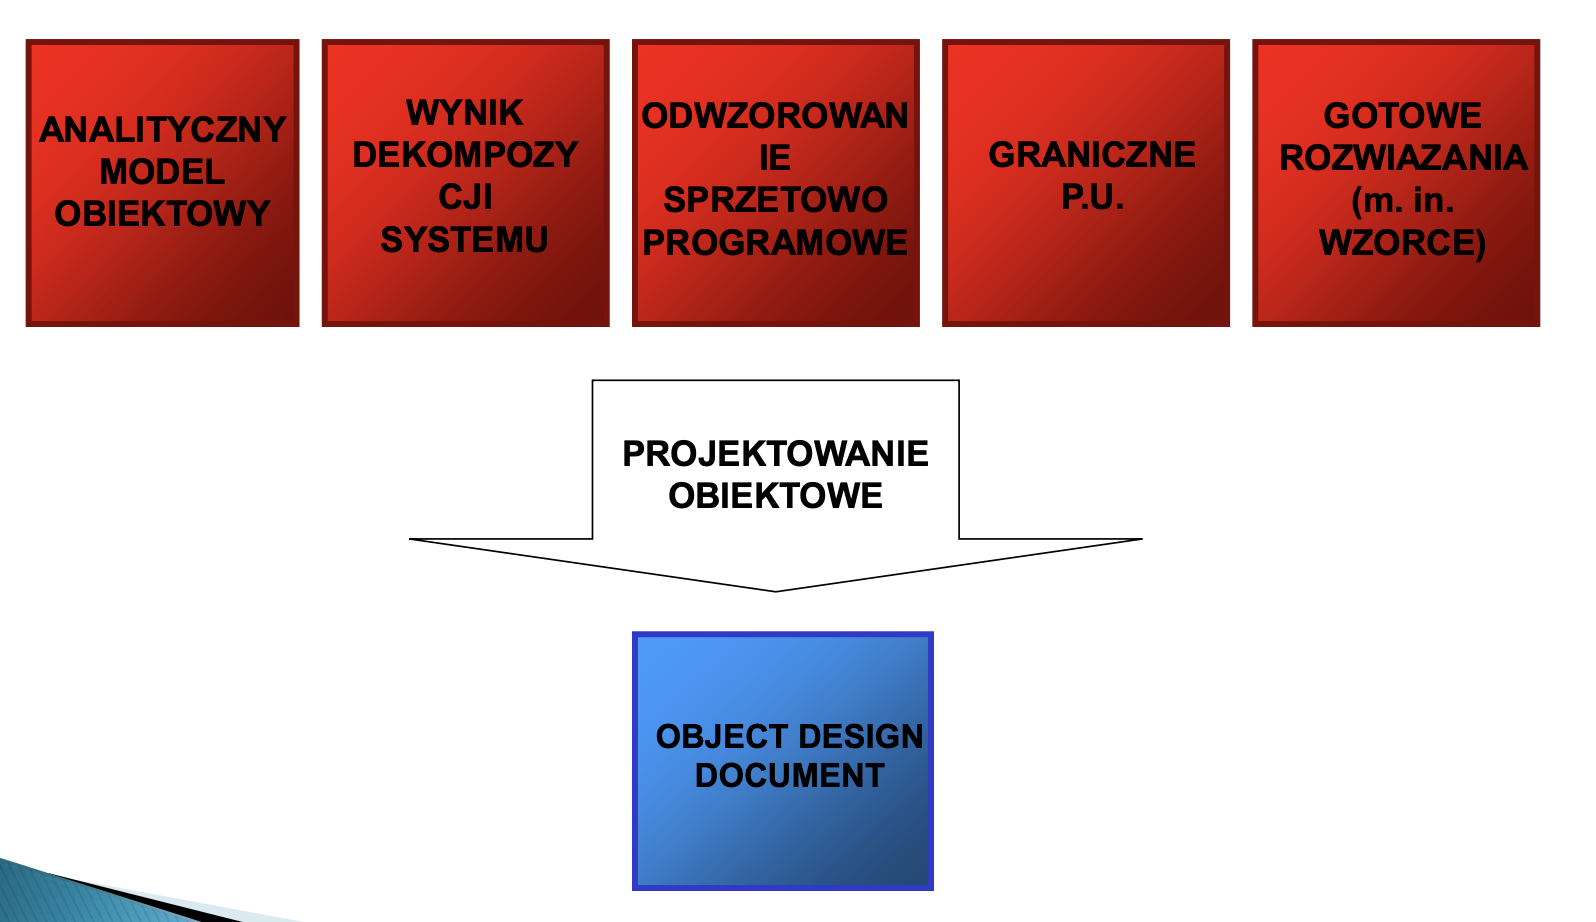
\includegraphics[width=\linewidth]{projektowanie_obiektow.png}
    \end{figure}

    \textbf{Etapy projektowania obiektów}
    \begin{itemize}
        \item wykorzystanie gotowych rozwiązań, którymi są zarówno
        gotowe produkty (komponenty) jak i wzorce projektowe;
        \item specyfikowanie usług;
        \item restrukturyzacja modelu obiektowego;
        \item optymalizacja modelu obiektowego;
    \end{itemize}

    \begin{figure}[H]
        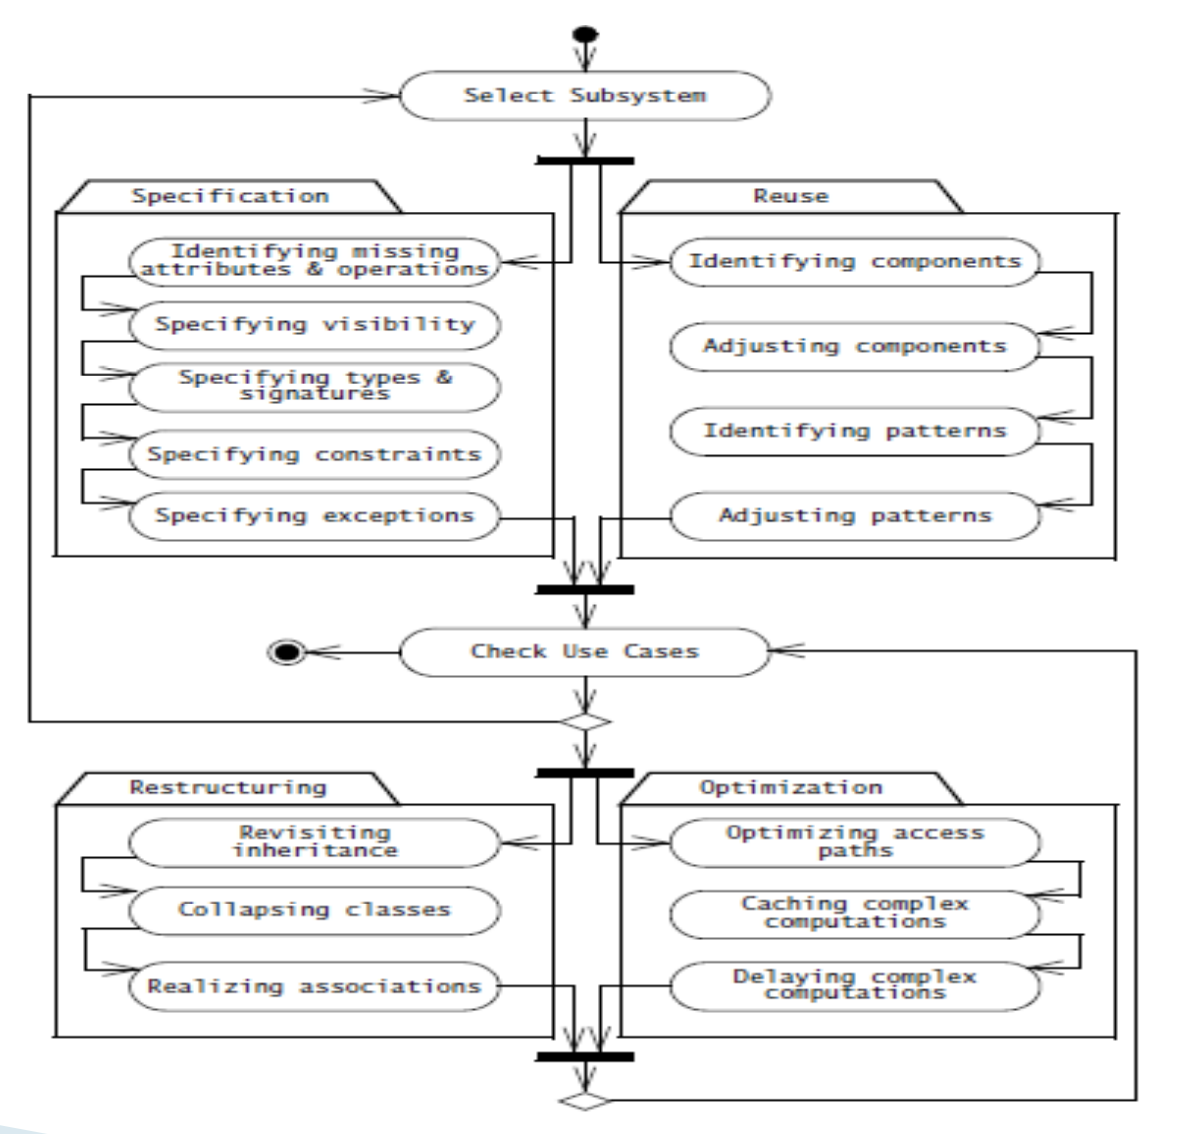
\includegraphics[width=\linewidth]{subsystem.png}
    \end{figure}

    Koncepcje wielokrotnego wykorzystywania gotowych rozwiązań:
    \begin{itemize}
        \item \textbf{obiekty aplikacyjne} - reprezentują koncepcje problemowe związane z tworzonym systemem.
        \item \textbf{obiekty realizacyjne} - reprezentują komponenty nie mające odpowiedników w
        dziedzinie aplikacyjnej, na przykład bazy danych czy obiekty interfejsu użytkownika.
        \item \textbf{dziedziczenie implementacyjne} - ma miejsce jeśli sięgamy po dziedziczenie z zamiarem wykorzystania
        gotowego kodu, mimo różnic koncepcyjnych pomiędzy powiązanymi klasami.
        \item \textbf{dziedziczenie specyfikacyjne} - ma odzwierciedlenie w taksonomii klas (reprezentuje podtypowanie).
        \item \textbf{delegowanie implementacji} - zamiast implementować set jako nadpisywanie metod hashtable, implementujemy go jako set korzystajacy z instancji hashtable z własnymi metodami.
        Rozwiązuje problemy dziedziczenia implementacyjnego: rozszerzalność, podtypowanie.
        \item \textbf{zasada zastępowania Liskov} - \textit{'Jeśli obiekt klasy S może stać się substytutem obiektu klasy T w
        dowolnym miejscu kodu, w którym oczekiwany jest obiekt klasy T, to klasa S jest podtypem klasy T.'}
        \item \textbf{wzorce projektowe} (obiektowe);
    \end{itemize}



    \subsection{Wzorce projektowe - poziom interakcji między klasami}
    \textbf{Wzorzec opisuje problem, który powtarza się wielokrotnie w danym środowisku, oraz podaje istotę
    jego rozwiązania.}

    \begin{itemize}
        \item Czy typowe problemy można rozwiązać w powtarzalny sposób?
        \item Czy te problemy można przedstawić w sposób abstrakcyjny, tak aby były pomocne
        w tworzeniu rozwiązań w róznych konkretnych kontekstach?
    \end{itemize}

    \begin{itemize}
        \item \textbf{Wzorce kreacyjne}
        \begin{itemize}
            \item abstrakcyjne metody tworzenia obiektów,
            \item uniezależnienie systemu od sposobu tworzenia obiektów.
        \end{itemize}
        \item \textbf{Wzorce strukturalne}
        \begin{itemize}
            \item sposób wiązania obiektów w struktury,
            \item właściwe wykorzystanie dziedziczenia i kompozycji.
        \end{itemize}
        \item \textbf{Wzorce behawioralne}
        \begin{itemize}
            \item algorytmy i przydział odpowiedzialności,
            \item opis przepływu kontroli i interakcji.
        \end{itemize}
    \end{itemize}

    \subsection{Koncepcje specyfikowania interfejsów}
    \begin{itemize}
        \item implementator (realize class), ekstender (refine class) i użytkownik (use class) klasy;
        \item typy, sygnatury (wektory/krotki typów parametrów i typu wyniku) i widzialność (public, private, protected, packet);
        \item kontrakty: niezmienniki, warunki wstępne i warunki końcowe;
        \item język OCL (Object Constraint Language) – ograniczenia
        \item OCL – zbiory, wielozbiory i ciągi;
        \item kwantyfikatory OCL;
    \end{itemize}

    \subsection{Aktywności specyfikowania interfejsów}
    \begin{itemize}
        \item identyfikowanie brakujących atrybutów i operacji;
        \item definiowanie widzialności i sygnatur;
        \item specyfikowanie kontraktów;
        \item dziedziczenie kontraktów;
    \end{itemize}



    \subsection{SOLID}


    \begin{tabular}{|c|c|}
        \hline
        S & Single responsibility principle\\
        & Klasa powinna mieć pojedyńczą
        odpowiedzialność.\\
        \hline
        O & Open/closed principle\\
        & Software powinien być otwarty na
        rozszerzenia a zamknięty na modyfikacje.\\
        \hline
        L & Liskov substitution principle\\
        \hline
        I & Interface segregation principle\\
        & Kilka konkretnych interfejsów jest lepszych
        niż jeden ogólny\\
        \hline
        D & Dependency inversion principle\\
        & Software powinien zależeć od abstrakcji a
        nie od konkretyzacji.\\
        \hline
    \end{tabular}

    \subsubsection{Single Resposibility Principle - SRP}
    \begin{itemize}
        \item Nigdy nie powinien istnieć więcej niż jeden powód do modyfikacji klasy.
        \item Im mniejsza i bardziej wyspecyfikowana klasa tym łatwiej ją nazwać.
        \item Łatwiejsze wprowadzanie zmian.
        \item Łatwiejsze testowanie i naprawa
    \end{itemize}

    Jak rozpoznać naruszenie SRP?
    \begin{itemize}
        \item Ilość linii kodu ( Class:LOC > 250)
        \item Za dużo
        zależności
        \item Słaba spojność
        \item Opis lub nazwa wymaga “i”
        \item Dużo zagnieżdżeń (ifów)
        \item Wymaga skomplikowanych testów
        \item Modyfikacja może zepsuć inne testy
    \end{itemize}



    \subsubsection{Zasada otwarte-zamknięte}
    \begin{itemize}
        \item klasa powinna być otwarta na rozbudowę, ale zamknięta do jej własnej modyfikacji
        \item możemy dodawać nowe pola i metody, ale bez zmiany w wewnętrznej strukturze
        \item zmiana istniejącej struktury może mieć wpływ na inne elementy
        \item hermetyzacja, dziedziczenie, polimorfizm, delegaty
        \item unikamy instrukcji warunkowych
    \end{itemize}

    \subsubsection{Zasada segregacji interfejsów}
    \begin{itemize}
        \item Związki między klasami powinny być ograniczone do minimum
        \item Klient klasy powinien mieć dostep tylko do tyh składowych klasy,
        których rzeczywiście potrzebuje
        \item Moduły wysokiego poziomu nie powinny
        zależeć od modułów niskopoziomowych.
        \item Obie grupy modułów powinny zależeć od
        abstrakcji
    \end{itemize}

    \subsubsection{Zasada odwracania zależności}
    'Hollywood Principle' - don't call us, we'll call you!

    \subsection{Wybrane wzorce kreacyjne}

    \subsubsection{Singleton}
    Cel:
    \begin{itemize}
        \item Zapewnienie, że klasa posiada jedną instancję wewnątrz całej aplikacji
        \item Stworzenie punktu dostępowego do tej instancji
    \end{itemize}

    \begin{figure}[H]
        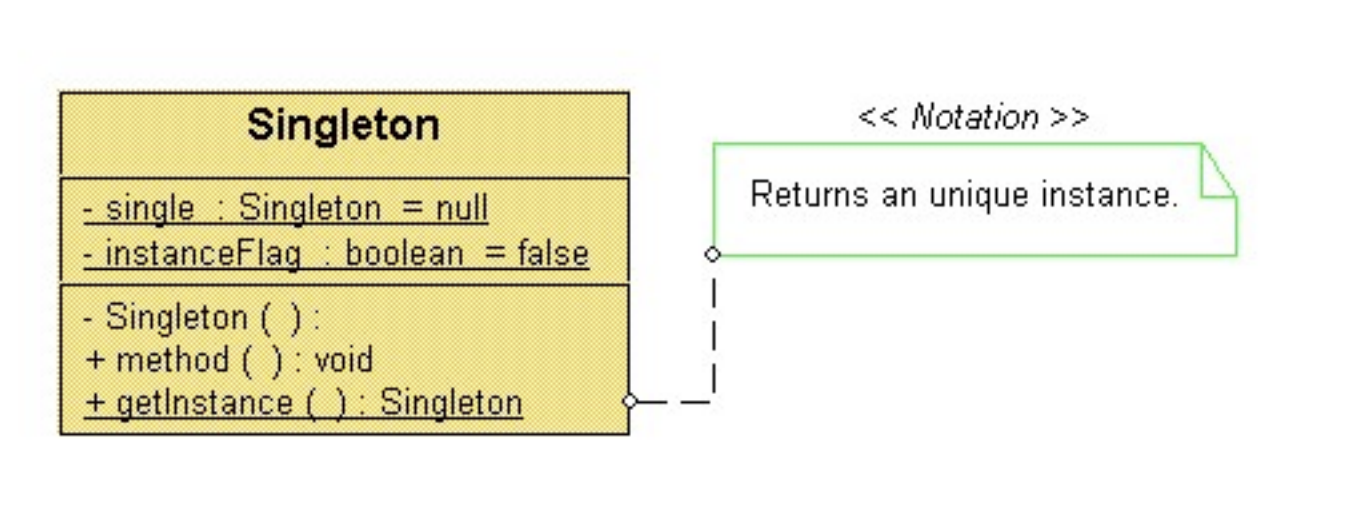
\includegraphics[width=\linewidth]{singleton.png}
    \end{figure}

    \subsubsection{Factory method}
    Cel:
    \begin{itemize}
        \item Zdefiniowanie interfejsu do tworzenia obiektów
        \item Umożliwienie przekazania odpowiedzialności za tworzenie obiektów
        do podklas
        \item Umożliwienie wyboru klasy i konstruktora użytego do utworzenia
        obiektu
    \end{itemize}

    \begin{figure}[H]
        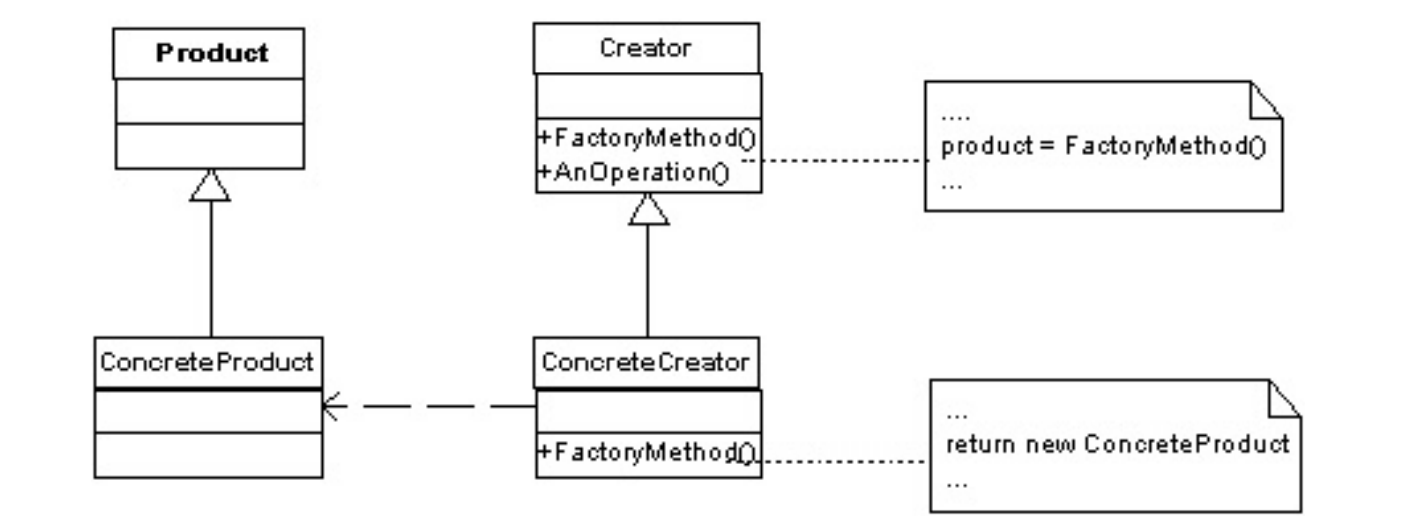
\includegraphics[width=\linewidth]{fac-met.png}
    \end{figure}


    \subsubsection{Builder}
    Cel:
    \begin{itemize}
        \item Odseparowanie sposobu reprezentacji i metody konstrukcji
        złożonych struktur obiektowych
        \item Wykorzystanie jednego mechanizmu konstrukcyjnego do tworzenia
        struktur o różnej reprezentacji
    \end{itemize}


    \begin{figure}[H]
        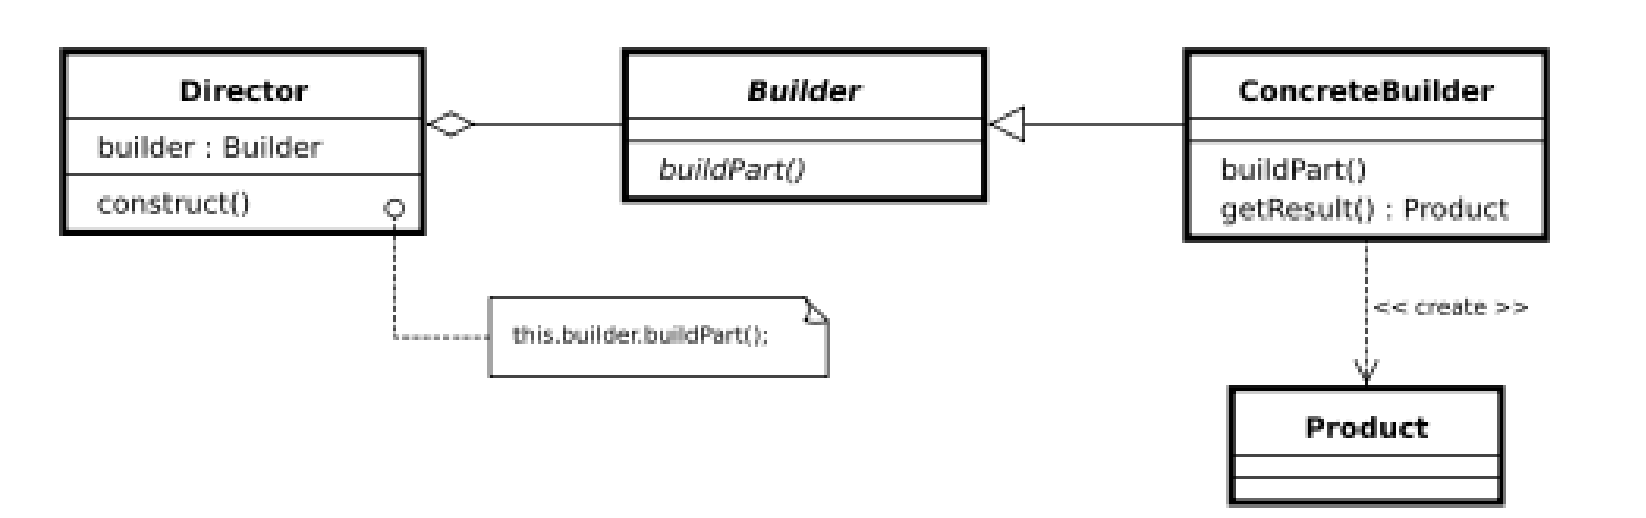
\includegraphics[width=\linewidth]{builder.png}
    \end{figure}



    \subsection{Wybrane wzorce strukturalne}

    \subsubsection{Adapter}
    Cel:
    \begin{itemize}
        \item Umożliwia współprace obiektów o niezgodnych typach
        \item Tłumaczy protokoły obiektowe
    \end{itemize}

    \begin{figure}[H]
        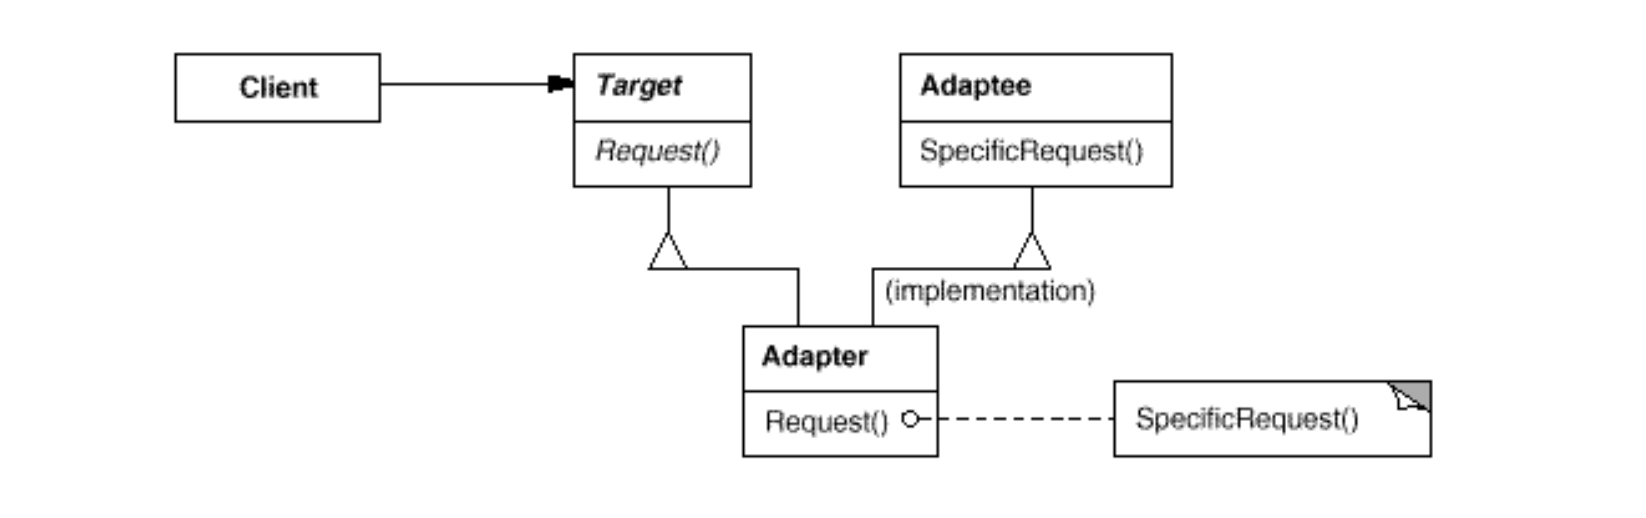
\includegraphics[width=\linewidth]{adapter.png}
    \end{figure}

    \subsubsection{Proxy}
    Cel:
    \begin{itemize}
        \item Dostarcza zamiennik obiektu w celu jego kontroli i ochrony
        \item Przezroczyste odsuniecie inicjalizacji obiektu w czasie
    \end{itemize}

    \begin{figure}[H]
        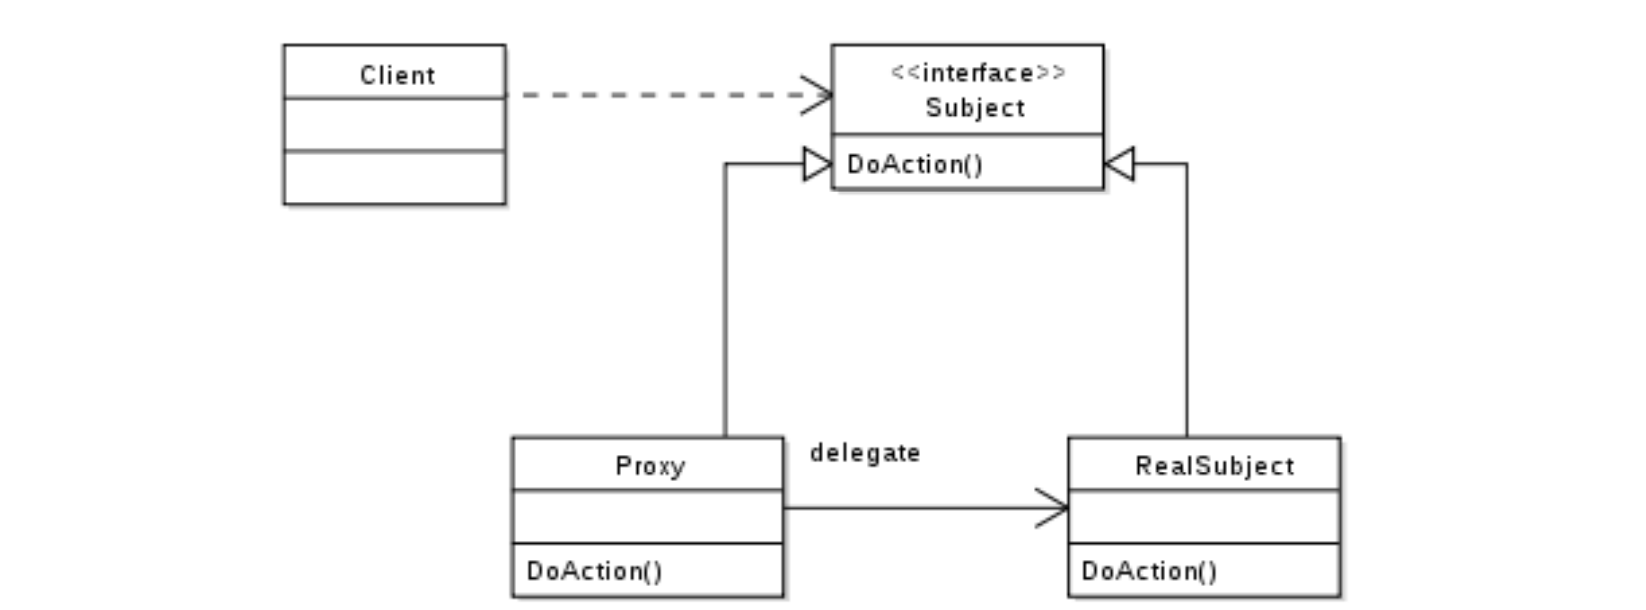
\includegraphics[width=\linewidth]{proxy.png}
    \end{figure}



    \subsubsection{Fasada}
    Cel:
    \begin{itemize}
        \item Dostarczenie jednorodnego interfejsu wyższego poziomu do zbioru
        rośnych interfejsów w systemie
        \item Ukrycie złożoności podsystemów przed klientem
    \end{itemize}

    \begin{figure}[H]
        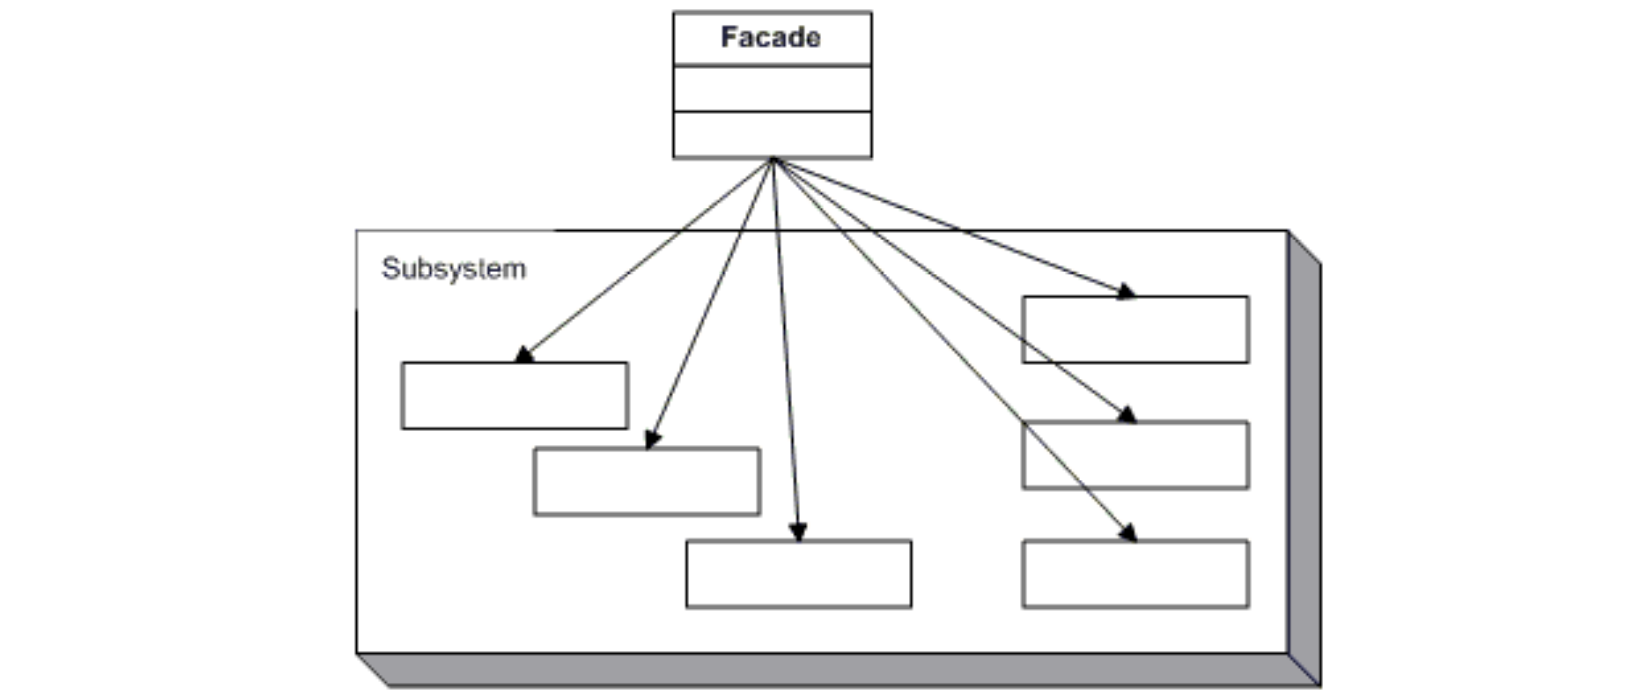
\includegraphics[width=\linewidth]{fasada.png}
    \end{figure}




    \subsection{Wybrane wzorce behawioralne}

    \subsubsection{Obserwator}
    \begin{itemize}
        \item Tworzy zależność typu jeden-wiele pomiędzy obiektami
        \item Informacja o zmianie stanu wyróżnionego obiektu jest przekazywana
        wszystkim pozostałym obiektom
    \end{itemize}

    \begin{figure}[H]
        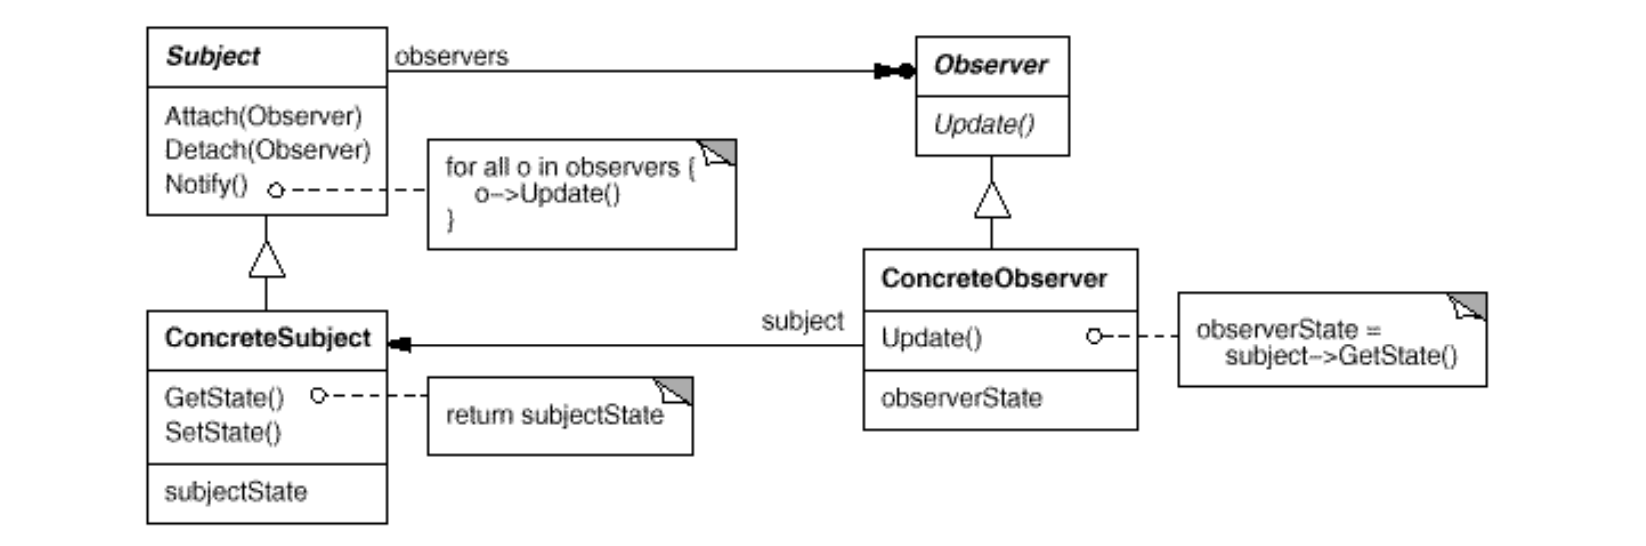
\includegraphics[width=\linewidth]{obserwator.png}
    \end{figure}


    \subsubsection{Command}
    \begin{itemize}
        \item Hermetyzacja poleceń do wykonania w postaci obiektów
        \item Umożliwienie parametryzacji klientów obiektami poleceń
        \item Wsparcie dla poleceń odwracalnych
    \end{itemize}

    \begin{figure}[H]
        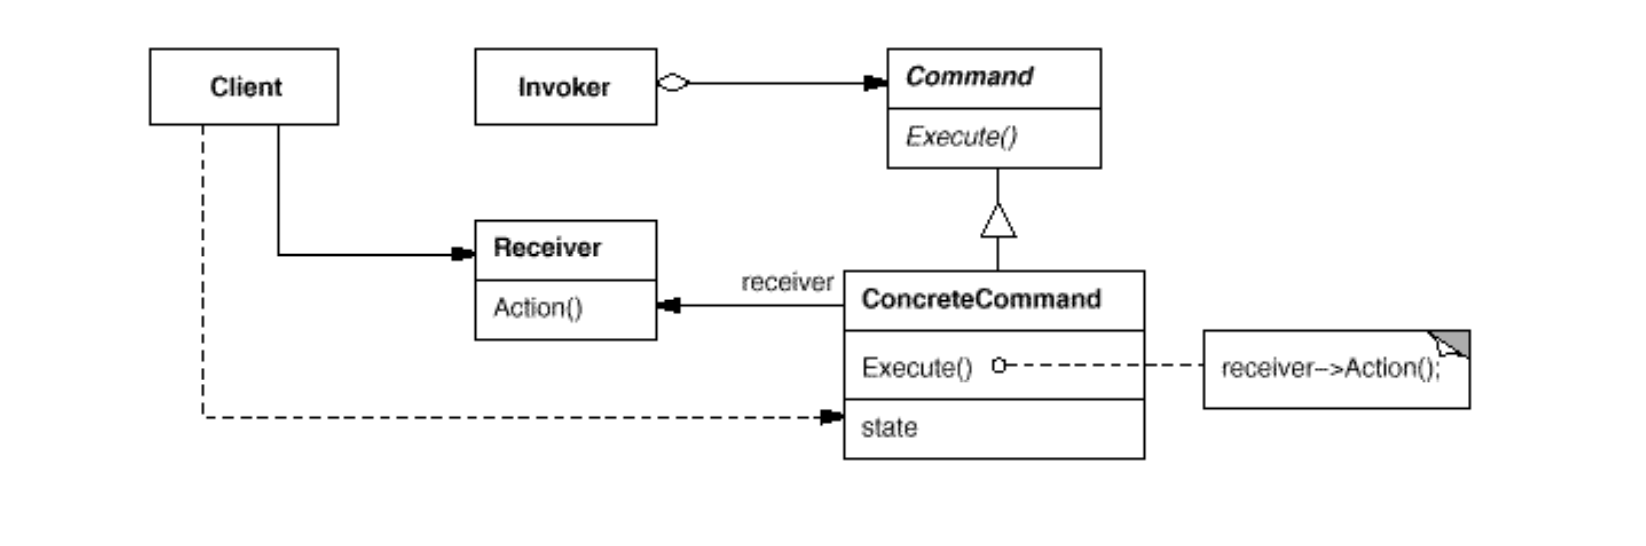
\includegraphics[width=\linewidth]{command.png}
    \end{figure}


    \subsubsection{Chain of responsibility}
    Cel:
    \begin{itemize}
        \item  Usunięcie powiązania pomiędzy nadawcą i odbiorcą żądania
        \item Umożliwienie wielu obiektom obsługi żądania
    \end{itemize}


    \begin{figure}[H]
        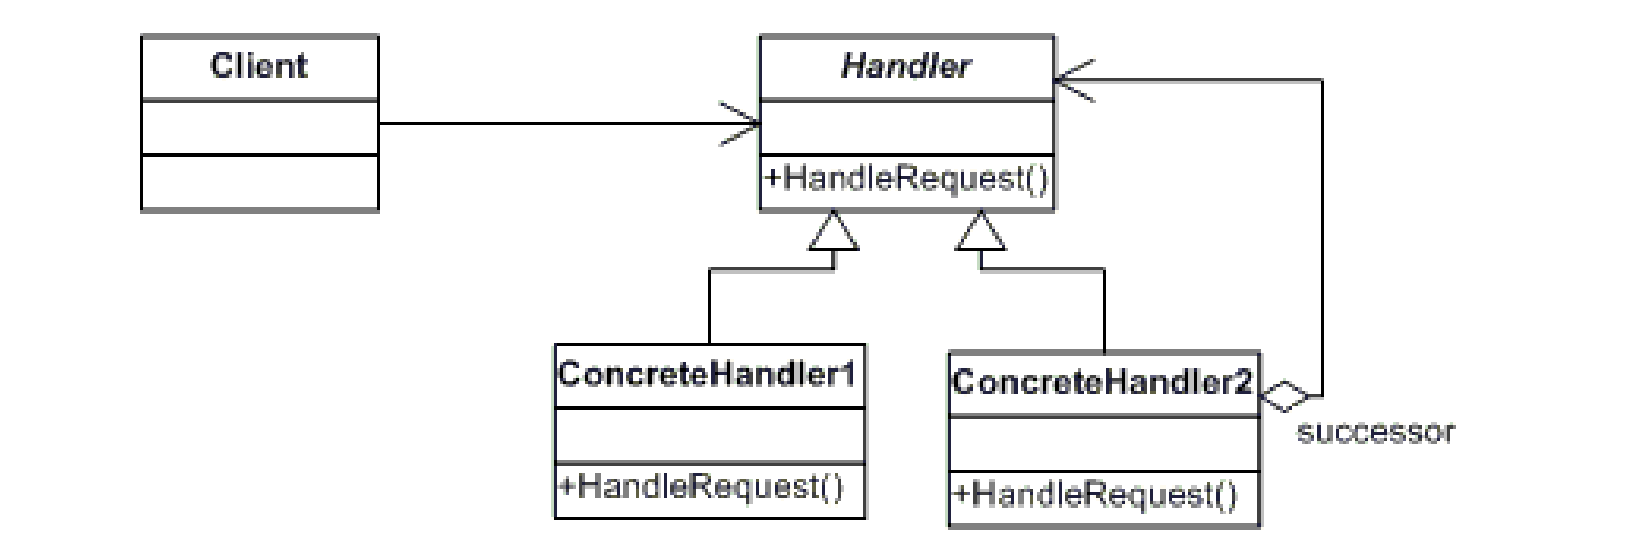
\includegraphics[width=\linewidth]{ch-o-r.png}
    \end{figure}


    \subsubsection{Iterator}
    Cel:
    \begin{itemize}
        \item Umożliwienie sekwencyjnego dostępu do elementów kolekcji bez
        ujawniania jej wewnętrznej implementacji
    \end{itemize}





    \begin{figure}[H]
        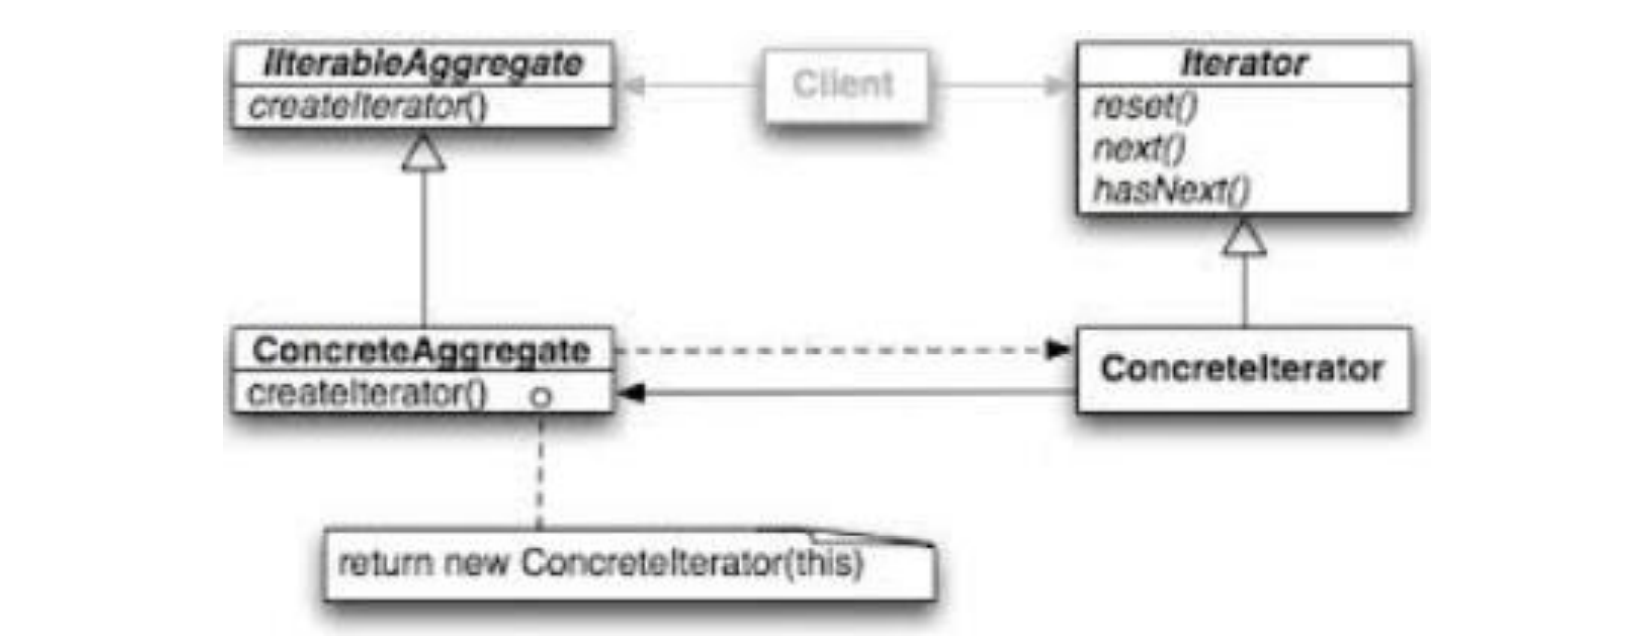
\includegraphics[width=\linewidth]{iterator.png}
    \end{figure}



    \subsection{Implementacja wzorców projektowych}
    Implementacja to transformowanie modelu w kod źródłowy.



    \begin{figure}[H]
        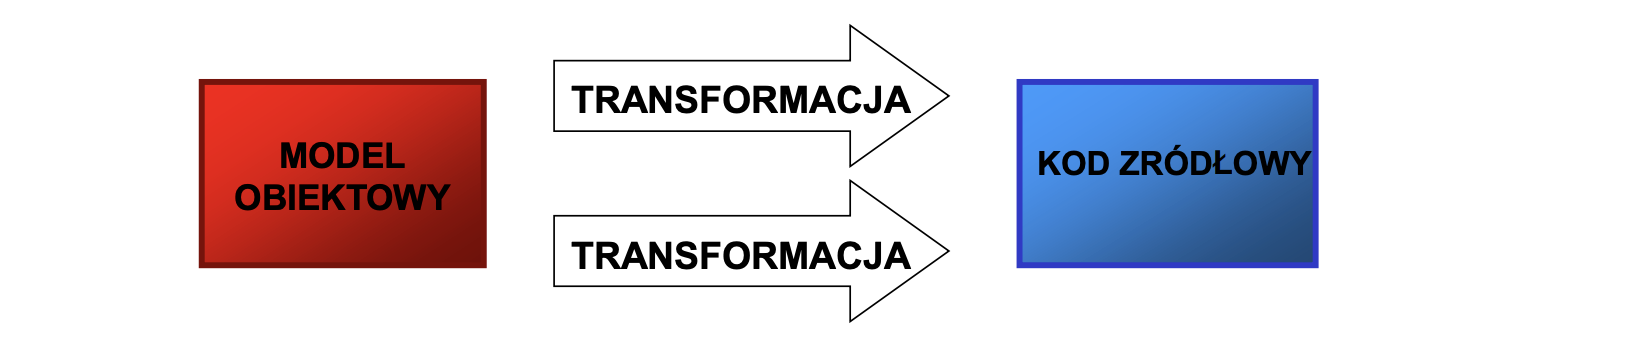
\includegraphics[width=\linewidth]{wzorce.png}
    \end{figure}

    Transformacje te wykonywane są w ramach następujących
    aktywności:
    \begin{itemize}
        \item optymalizowanie modelu
        \item realizowanie skojarzeń
        \item definiowanie wyjątków związanych z naruszeniem kontraktów
        \item odwzorowywane modeli klas w schematy przechowywania danych
    \end{itemize}

    Zasady transformacji:
    \begin{itemize}
        \item każda transformacja powinna dotyczyć tylko jednego,
        ściśle określonego kryterium;
        \item każda transformacja musi mieć charakter lokalny;
        \item każda transformacja powinna być izolowana od
        innych zmian;
        \item każda transformacja musi być poddana weryfikacji;
    \end{itemize}


    Najczęściej wykonywane aktywności (transformacje):
    \begin{itemize}
        \item optymalizowanie modelu obiektowego;
        \item odwzorowywanie skojarzeń w kolekcje;
        \item odwzorowywanie kontraktów w wyjątki;
        \item odwzorowywanie modelu obiektowego w schematy
        bazy danych;
    \end{itemize}

    Typy transformacji
    \begin{itemize}
        \item Transformacja modelu
        \begin{itemize}
            \item ograniczona jest do samego modelu
            \item celem jest uproszczenie lub zoptymalizowanie istniejącego modelu
        \end{itemize}
        \item Inżynieria postępująca
        \begin{itemize}
            \item tworzenie szablonów kodu źródłowego odpowiadającego modelowi obiektowemu
        \end{itemize}
    \end{itemize}

    \subsubsection{Paradygmaty programowania}

    Paradygmat:
    \begin{itemize}
        \item wzorzec lub najogólniejszy
        model lub jako wzorcowy przykład.
        \item zbiór pojęć i teorii tworzących podstawy danej nauki.
    \end{itemize}


    Podstawowe założenia paradygmatu:
    \begin{itemize}
        \item Abstrakcja\\
        System rozumiany jest jako układ obiektów . Każdy
        obiekt w systemie można rozpatrywać jako model
        abstrakcyjnego elementu, który może:
        \begin{itemize}
            \item opisywać i zmieniać swój stan,
            \item komunikować się z innymi obiektami w systemie,
            \item wykonywać pewne czynności na rzecz innych obiektów,
            \item bez ujawniania, w jaki sposób zaimplementowano
            dane cechy.
        \end{itemize}
        \item Enkapsulacja\\
        \begin{itemize}
            \item Polega na ukrywaniu szczegółów implementacji.
            \item Ma to spowodować, że obiekt nie może zmieniać
            stanu wewnętrznego innych obiektów w
            nieoczekiwany sposób.
            \item Tylko wewnętrzne metody obiektu są uprawnione
            do zmiany jego stanu.
            \item Każdy typ obiektu dostarcza innym obiektom swój
            "interfejs", który określa dopuszczalne metody współpracy.
        \end{itemize}
        \item Polimorfizm\\
        \begin{itemize}
            \item Polimorfizm w programowaniu obiektowym to
            wykazywanie różnych form działania podczas
            wywoływania metody w zależności od tego jakiego
            typu obiekt jest wskazywany przez wskaźnik lub
            referencję.
            \item Referencje i kolekcje obiektów mogą dotyczyć
            obiektów różnego typu, a wywołanie metody dla
            referencji spowoduje zachowanie odpowiednie dla
            pełnego typu obiektu wywoływanego.
        \end{itemize}
        \item Dziedziczenie\\
        \begin{itemize}
            \item Dziedziczenie porządkuje i wspomaga polimorfizm i
            enkapsulację.
            \item Osiąga to dzięki umożliwieniu definiowania i
            tworzenia specjalizowanych obiektów na podstawie
            bardziej ogólnych.
            \item Dla obiektów specjalizowanych nie trzeba
            redefiniować całej funkcjonalności, lecz tylko tę,
            której nie mają obiekty ogólniejsze.
        \end{itemize}
    \end{itemize}

    GRASP - General Responsibility Assignment Software Patterns odpowiada na pytania w zakresie odpowiedzialności.
    \begin{itemize}
        \item Creator - określa kiedy podany obiekt powinien tworzyć inny obiekt, tzn. B powinien tworzyć A, jeśli:
        \begin{itemize}
            \item B agreguje A,
            \item B operuje na danych obiektu A,
            \item B używa bezpośrednio A,
            \item B dostarcza informacji niezbędnej do utworzenia A
        \end{itemize}
        \item Information Expert\\
        Programista powinien delegować nową
        odpowiedzialność (nowe funkcje) do obiektów, które
        zawierają najwięcej informacji/danych
        pozwalających zrealizować nową funkcjonalność.
        Istotne jest więc określenie, jakie dane są niezbędne
        do wypełnienia danej odpowiedzialności. Dopiero w
        tym momencie można powiedzieć, który obiekt
        powinien mieć przypisaną nową funkcjonalność
        \item Controller\\
        Programista powinien delegować zadania z interfejsu
        użytkownika do kontrolera.
        Zadaniem kontrolera jest: odbieranie informacji od UI,
        wykonywanie operacji oraz zwracanie ich wyników
        do UI. Kontroler powinien delegować zadania w głąb
        systemu
        \item Low Coupling\\
        Klasy powinny być od siebie jak najbardziej
        niezależne. Zmiana w jednej klasie powinna
        prowadzić do jak najmniejszej ilości zmian w innych
        klasach.
        \item High Cohesion\\
        Obiekt powinien skupiać się na jednej
        odpowiedzialności. Jego odpowiedzialność nie
        powinna być rozmyta, gdyż nie wiadomo
        wtedy dlaczego obiekt istnieje w systemie
        \item Polymorphism
        \item Pure Fabrication\\
        W systemie mogą istnieć operacje, których nie
        da się przypisać do żadnego obiektu
        dziedziny. Prowadzi to do powstawania w
        systemie obiektów, które nie reprezentują
        żadnego obiektu dziedziny, a kondensują
        funkcje udostępniane na rzecz innych
        obiektów.
        Zapewniają zbiór usług na rzecz innych
        obiektów, np.: dostęp do repozytorium.
        \item Indirection\\
        Aby zapewnić low coupling często zachodzi potrzeba
        dodania mediatora w komunikacji między biektami.
        Jego zadaniem jest jedynie wymiana informacji
        między obiektami. Taki obiekt deleguje zadania z
        jednego obiektu na rzecz drugiego. Projektowanie
        systemu z użyciem mediatora wpływa na poprawę
        hermetyzacji elementów systemu.
        Model MVC jest dobrym tego przykładem astosowania
        tej zasady. Kontroler jest mediatorem, co izoluje
        interfejs użytkownika od modelu.
        \item Protected variations\\
        Zasada mówiąca o zakresie modyfikacji w systemie
        wymaganym przez określoną zmianę. W systemie
        powinno się identyfikować punkty niestabilności i
        budować interfejsy wokół tych punktów.
        To ograniczy zakres zmian w przypadku, gdyby
        okazało się, że podany punkt niestabilności systemu
        wymaga zmian.
    \end{itemize}




    \subsubsection{Metazasady}


    \begin{itemize}
        \item Don't repeat yourself - DRY\\
        Jedno miejsce w systemie, na pojedynczą informację,
        co ułatwia późniejsze zmiany.
        Inna nazwa to Single Source Of Truth (SSOT), każda
        informacja w systemie powinna być przechowywana
        dokładnie raz, bo ułatwia to jej modyfikację.
        \item Keep it simple, stupid - KISS\\
        W projektowaniu interfejsów powyższą zasadę można
        nazwać zasadą najmniejszego zaskoczenia, czyli
        fragment kodu powinien robić dokładnie to co ma
        robić.
        Czasem trzeba wybrać, czy dany fragment kodu
        napisać z wykorzystaniem wzorca projektowego czy
        prostej konstrukcji.
    \end{itemize}


\end{document}
